\chapter{LHC-ATLAS実験}
\thispagestyle{empty}
\label{chap:2}
LHC-ATLAS実験は、LHC加速器を用いた陽子陽子衝突によって生成された粒子をATLAS検出器を用いて測定する世界最大規模の素粒子実験である~\cite{TR:01}。標準模型の精密測定や新しい物理の探索を目的として行われている。
本章では、LHC~の概要及び~ATLAS~実験と各検出器について述べる。

\section{LHC 加速器}
スイスのジュネーブにある欧州原子核研究機構~(CERN)~の地下に建設された陽子陽子衝突型加速器~(LHC)~は、周長~27~km~のハドロンコライダーである。陽子バンチの衝突は~25~ns~おきに行われており、その頻度は~40~MHz~である。LHC~で加速する粒子は陽子であるため、電子陽電子コライダーと比べ粒子がリング内を回る時のシンクロトロン放射光によるエネルギー損失が少ないことが特徴の一つである。トンネル内に多数の超伝導電磁石を並べて強力な磁場を作り出し、高エネルギーでの陽子陽子衝突を実現させている。

LHC~では、標準模型の精密検証や新物理の発見を目指した~ATLAS~\cite{URL:13}と~CMS~\cite{URL:14}、重イオン衝突実験~ALICE~\cite{URL:15}、およびフレーバー物理に特化した~LHCb~\cite{URL:16}の~4~つの実験が行われている。\figref{fig:lhc}は~LHC~全体の外観および各実験の衝突点について示したものである。

LHC~の運用スケジュールの詳細について説明する。LHC~は~2010~年から本格的な運転~(Run~1)~を開始した。
Run~1は2010~年から2012~年まで行われた。その後、2013~年から2015~年初頭までの~Long~Shutdown~1~(LS1)~を経て~2018~年終わりまでの第二期運転~(Run~2)~が施行された。そして二度目のアップグレード期間~Long~Shutdown~2~(LS2)~が~2021~年終わりまで取られ、2022~年から第三期運転~(Run~3)~が行われる予定である。Run~3~の後には、より高いルミノシティでの~LHC~の運用が行われ、High-Luminosity~LHC~(HL-LHC)~として~2029~年から運転が施行される予定である。\tbref{tb:LHC}に各運転の詳細について示す。

時間$dt$における瞬間ルミノシティは
\begin{align}
    L = \frac{1}{\sigma}\frac{dN}{dt} \label{eq:lumi}
\end{align}
と表す。
ここで$\sigma$は陽子衝突の断面積、$dN$は事象数である。
通常、単位には$\rm{cm}^{-2}\rm{s}^{-1}$が用いられる。
\equref{eq:ilumi}で示すような時間に対するルミノシティの積分を積算ルミノシティ$L_{\rm{int}}$で表し
\begin{align}
    L_{\rm{int}} = \int{Ldt} \label{eq:ilumi}
\end{align}
となる。
観測されるデータ量は$L_{\rm{int}}$に比例し、単位には$\rm{fb}^{-1}$が用いられる。
\begin{table}[tb]
	\centering
	\begin{tabular}{c|cccc}\hline
	    \multirow{2}{*}{LHC Run} & \multirow{2}{*}{期~間} & 重心系エネルギー & 瞬間ルミノシティ & 積算ルミノシティ \\ 
	     &  & [TeV] & [$\rm{cm}^{-2}\rm{s}^{-1}$] & [$\rm{fb}^{-1}$] \\ \hline\hline
		Run 1 & $\rm{2010\sim\rm2012}$ & $\rm{7\sim8}$ & $0.77\times10^{34}$ & $28.26$ \\ \hline
		Run 2 & $\rm{2015\sim2018}$ & $\rm{13}$ & $2\times10^{34}$ & $184.26$ \\ \hline
		Run 3 & $\rm{2022\sim2025}$ & $\rm{13.6}$ & $2\times10^{34}$ & 約$350$ \\\hline
		HL-LHC & $\rm{2029\sim}$ & $\rm{14}$ & $5\sim7.5\times10^{34}$ & 約$3000\sim4000$ \\ \hline
	\end{tabular}
	\caption[LHC の各運転における詳細]{LHC~の各運転における詳細~\cite{URL:18,URL:17}。Run~3~以降については現在予定されている設定値を記している。積算ルミノシティは~LHC~で供給されるビームに基づいて計算している。}
    \label{tb:LHC}
\end{table} 
\begin{figure}[tbp]
        \centering   
        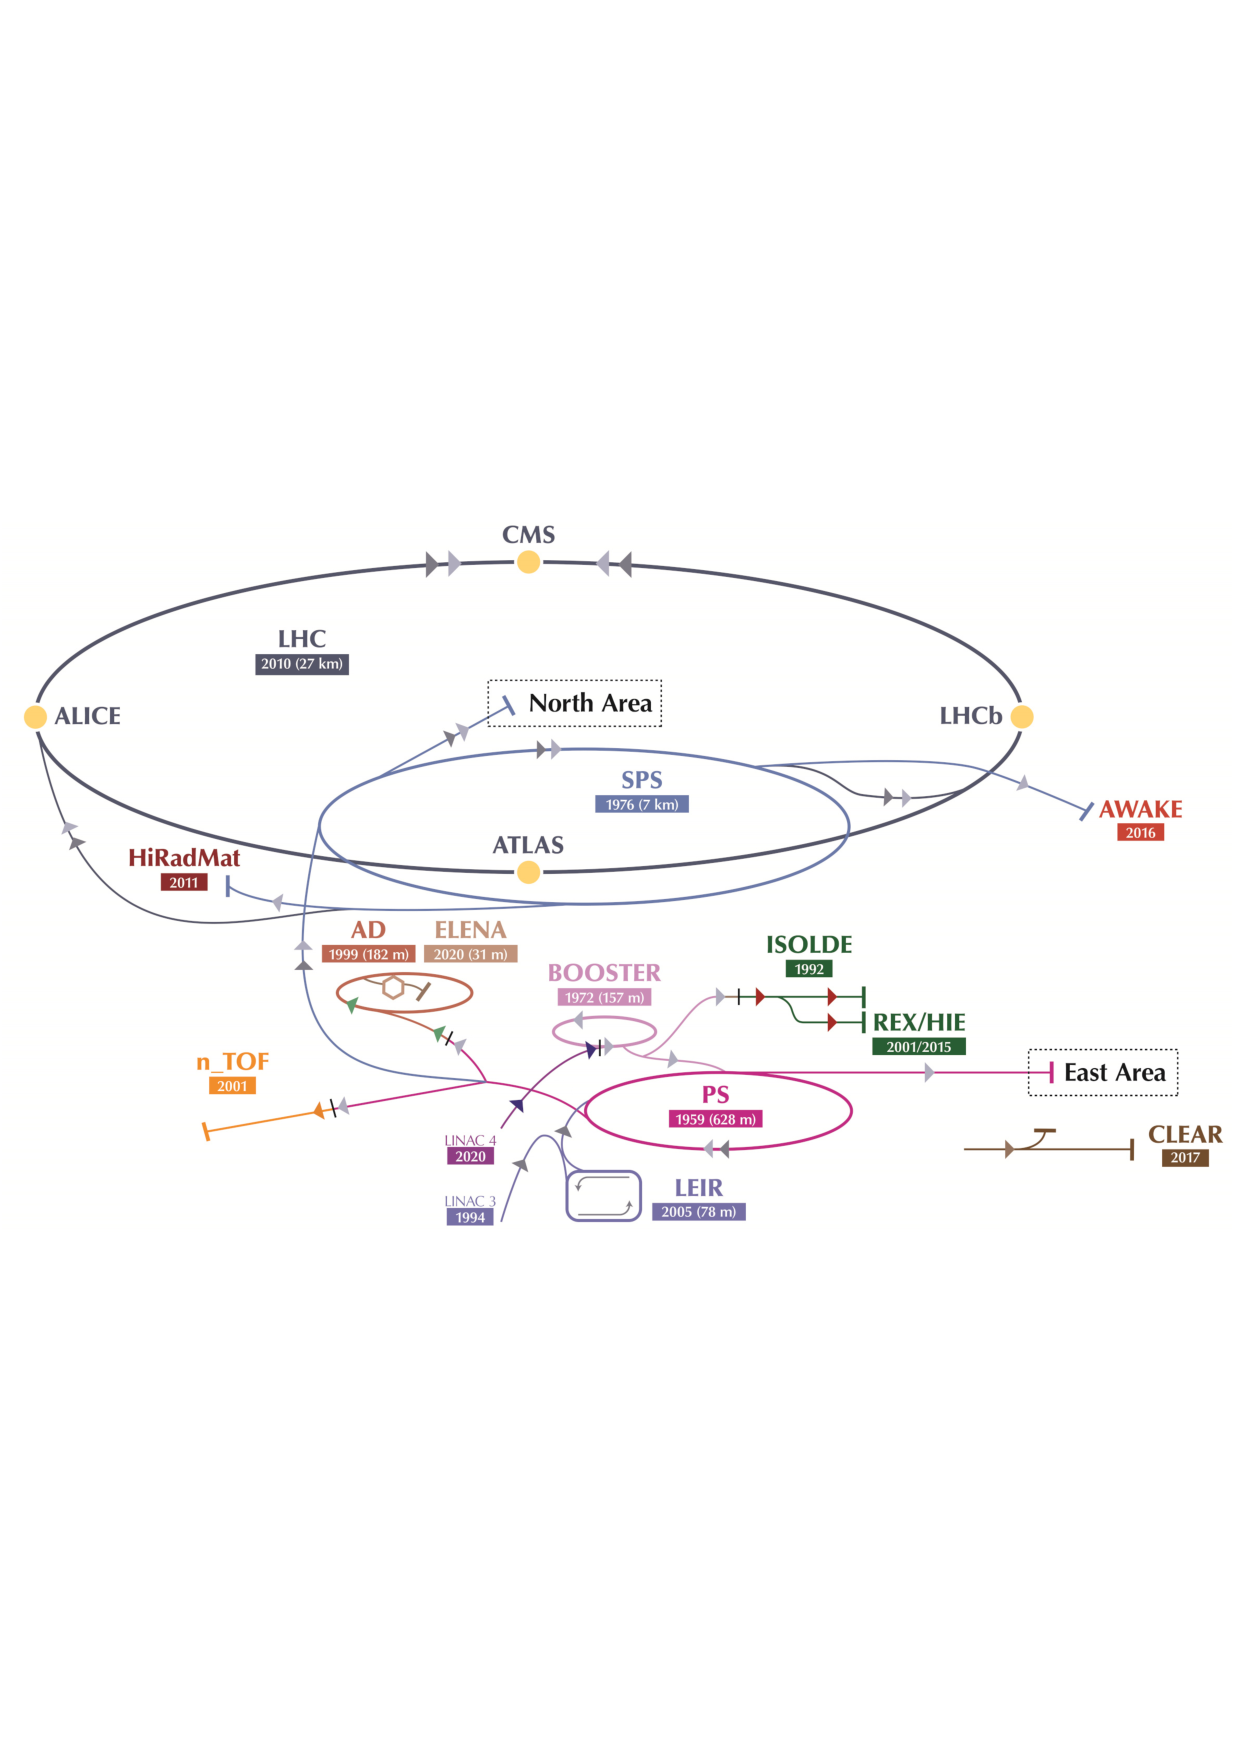
\includegraphics[width=0.8\textwidth]{img/jpeg/lhclhc.pdf}
        \caption[LHC 加速器の全体像]{LHC~加速器の全体像~\cite{URL:01}。LHC~並びに~LHC~の前段加速器の詳細を示している。LHC~には、ATLAS,~ALICE,~CMS,~LHCb~の~4~つの検出器が設置されている。}\label{fig:lhc}
\end{figure}
\section{ATLAS~実験}
ATLAS~実験は~LHC~の衝突点に設置されたATLAS検出器を用いて陽子陽子衝突から~TeV~スケールまでの高エネルギー物理事象の探索を行う実験である。2012~年には、同じ~LHC~の~CMS~実験と共にヒッグス粒子を発見し、標準理論の完成に向けて大きく貢献した~\cite{TR:03,TR:03a}。
本節では、ATLAS~実験の詳細について記していく。
\subsection{ATLAS~検出器}
ATLAS~検出器は、直径~22~m、長さ~44~m~の円筒形で、総重量は~7000~t~という大型汎用検出器である。\figref{fig:atlasdet}にATLAS検出器の全体図を示した。検出器は内側から内部飛跡検出器、電磁カロリメータ、ハドロンカロリメータ、ミューオン検出器という構成になっており、検出器の間には粒子を曲げるための超電導マグネットが設置されている。検出器は広範囲をカバーし、多様な検出器を組み合わせて利用することで高頻度の事象を逃すことなく処理するシステムが構築されている。\figref{fig:disp}は、衝突点より生成された粒子の各検出器における反応の様子を示したイベントディスプレイである。それぞれの検出器の特性をもとに各検出器で様々な粒子の識別を行う。

\begin{figure}[tbp]
    \centering   
    \includegraphics[width=0.9\textwidth,page=1]{img/pdf/ATLAS.pdf}
    \caption[ATLAS 検出器の全体図]{ATLAS 検出器の全体図~\cite{TR:01}。直径~25~m,~長さ~44~m,~重さ~7000~t~の大型汎用検出器。}\label{fig:atlasdet}
\end{figure}

\begin{figure}[htbp]
    \centering   
    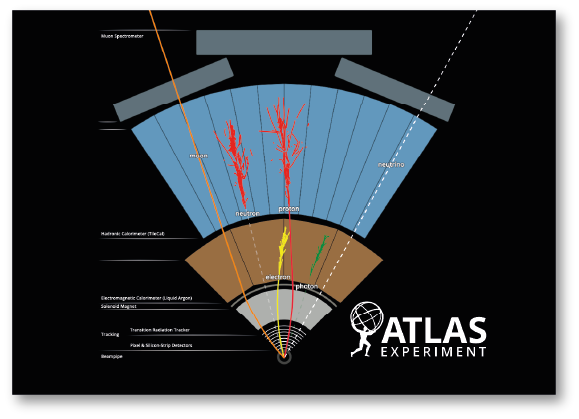
\includegraphics[width=0.85\textwidth]{img/jpeg/how.png}
    \caption[ATLAS~検出器の断面図と通過する粒子のふるまい]{ATLAS~検出器の断面図と通過する粒子のふるまい~\cite{URL:02}。電磁カロリメータでは電子や光子、ハドロンカロリメータでは陽子や中性子、ミューオン検出器ではミューオンの検出を行う。}
    \label{fig:disp}
\end{figure}

\subsection{ATLAS~座標系}
ATLAS~で一般的に利用されている座標系について説明する。\figref{fig:cood}にATLAS検出器のビーム衝突点を原点とした座標系を示した。直交座標系では検出器中心を原点にとり、ビーム軸方向を$z$軸、地面から垂直上方向を$y$軸、LHC~リングの中心を正方向を$x$軸として定義する。またATLAS~では検出器が円筒形のため極座標系が用いられることが多い。任意の$z$座標における動径方向を$R$、方位角方向を$\phi$、極角方向を$\theta$で表す。
$\theta$方向を表す際には擬ラピディティ$\eta$というパラメータ、\equref{eq:eta}がよく用いられる。
擬ラピディティは、ローレンツ変換において不変であるため素粒子実験ではしばしば利用されるパラメータである。
擬ラピディティにより領域を区分することができ、ミューオン検出器においては円筒型の側面部にあたる
$|\eta| < 1.05$をバレル領域、円筒型の底面部にあたる$|\eta| > 1.05$をエンドキャップ領域としている。
また、$\eta>0$の領域を~A-Side、$\eta<0$の領域を~C-Side~と呼んでいる。

\begin{align}
    \eta = -\rm{ln}\left(\rm{tan}\frac{\theta}{2}\right) \label{eq:eta}
\end{align}

粒子のエネルギーや運動量を表す際には、ビーム軸に垂直な成分である横方向エネルギー~($E_{\rm{T}}$)、横方向運動量~($p_{\rm{T}}$)~を利用する。陽子陽子衝突実験において、衝突するクォークやグルーオンの$z$軸方向のエネルギー・運動量には陽子内のパートン分布により不定のため保存則を用いることはできない。一方で、ビーム軸に垂直な方向にはエネルギーおよび運動量の保存則が成立する。従って$E_{\rm{T}}$や$p_{\rm{T}}$は解析において利用されることが多い。またビーム軸に垂直な方向成分の保存則を用いると、ニュートリノ等のATLAS検出器で観測できなかった粒子によるエネルギーの~2~次元のベクトル和を得ることができる。この見えないエネルギーの和を消失横方向エネルギー~(MET)~と呼ぶ。

\begin{figure}[tbp]
    \centering  
    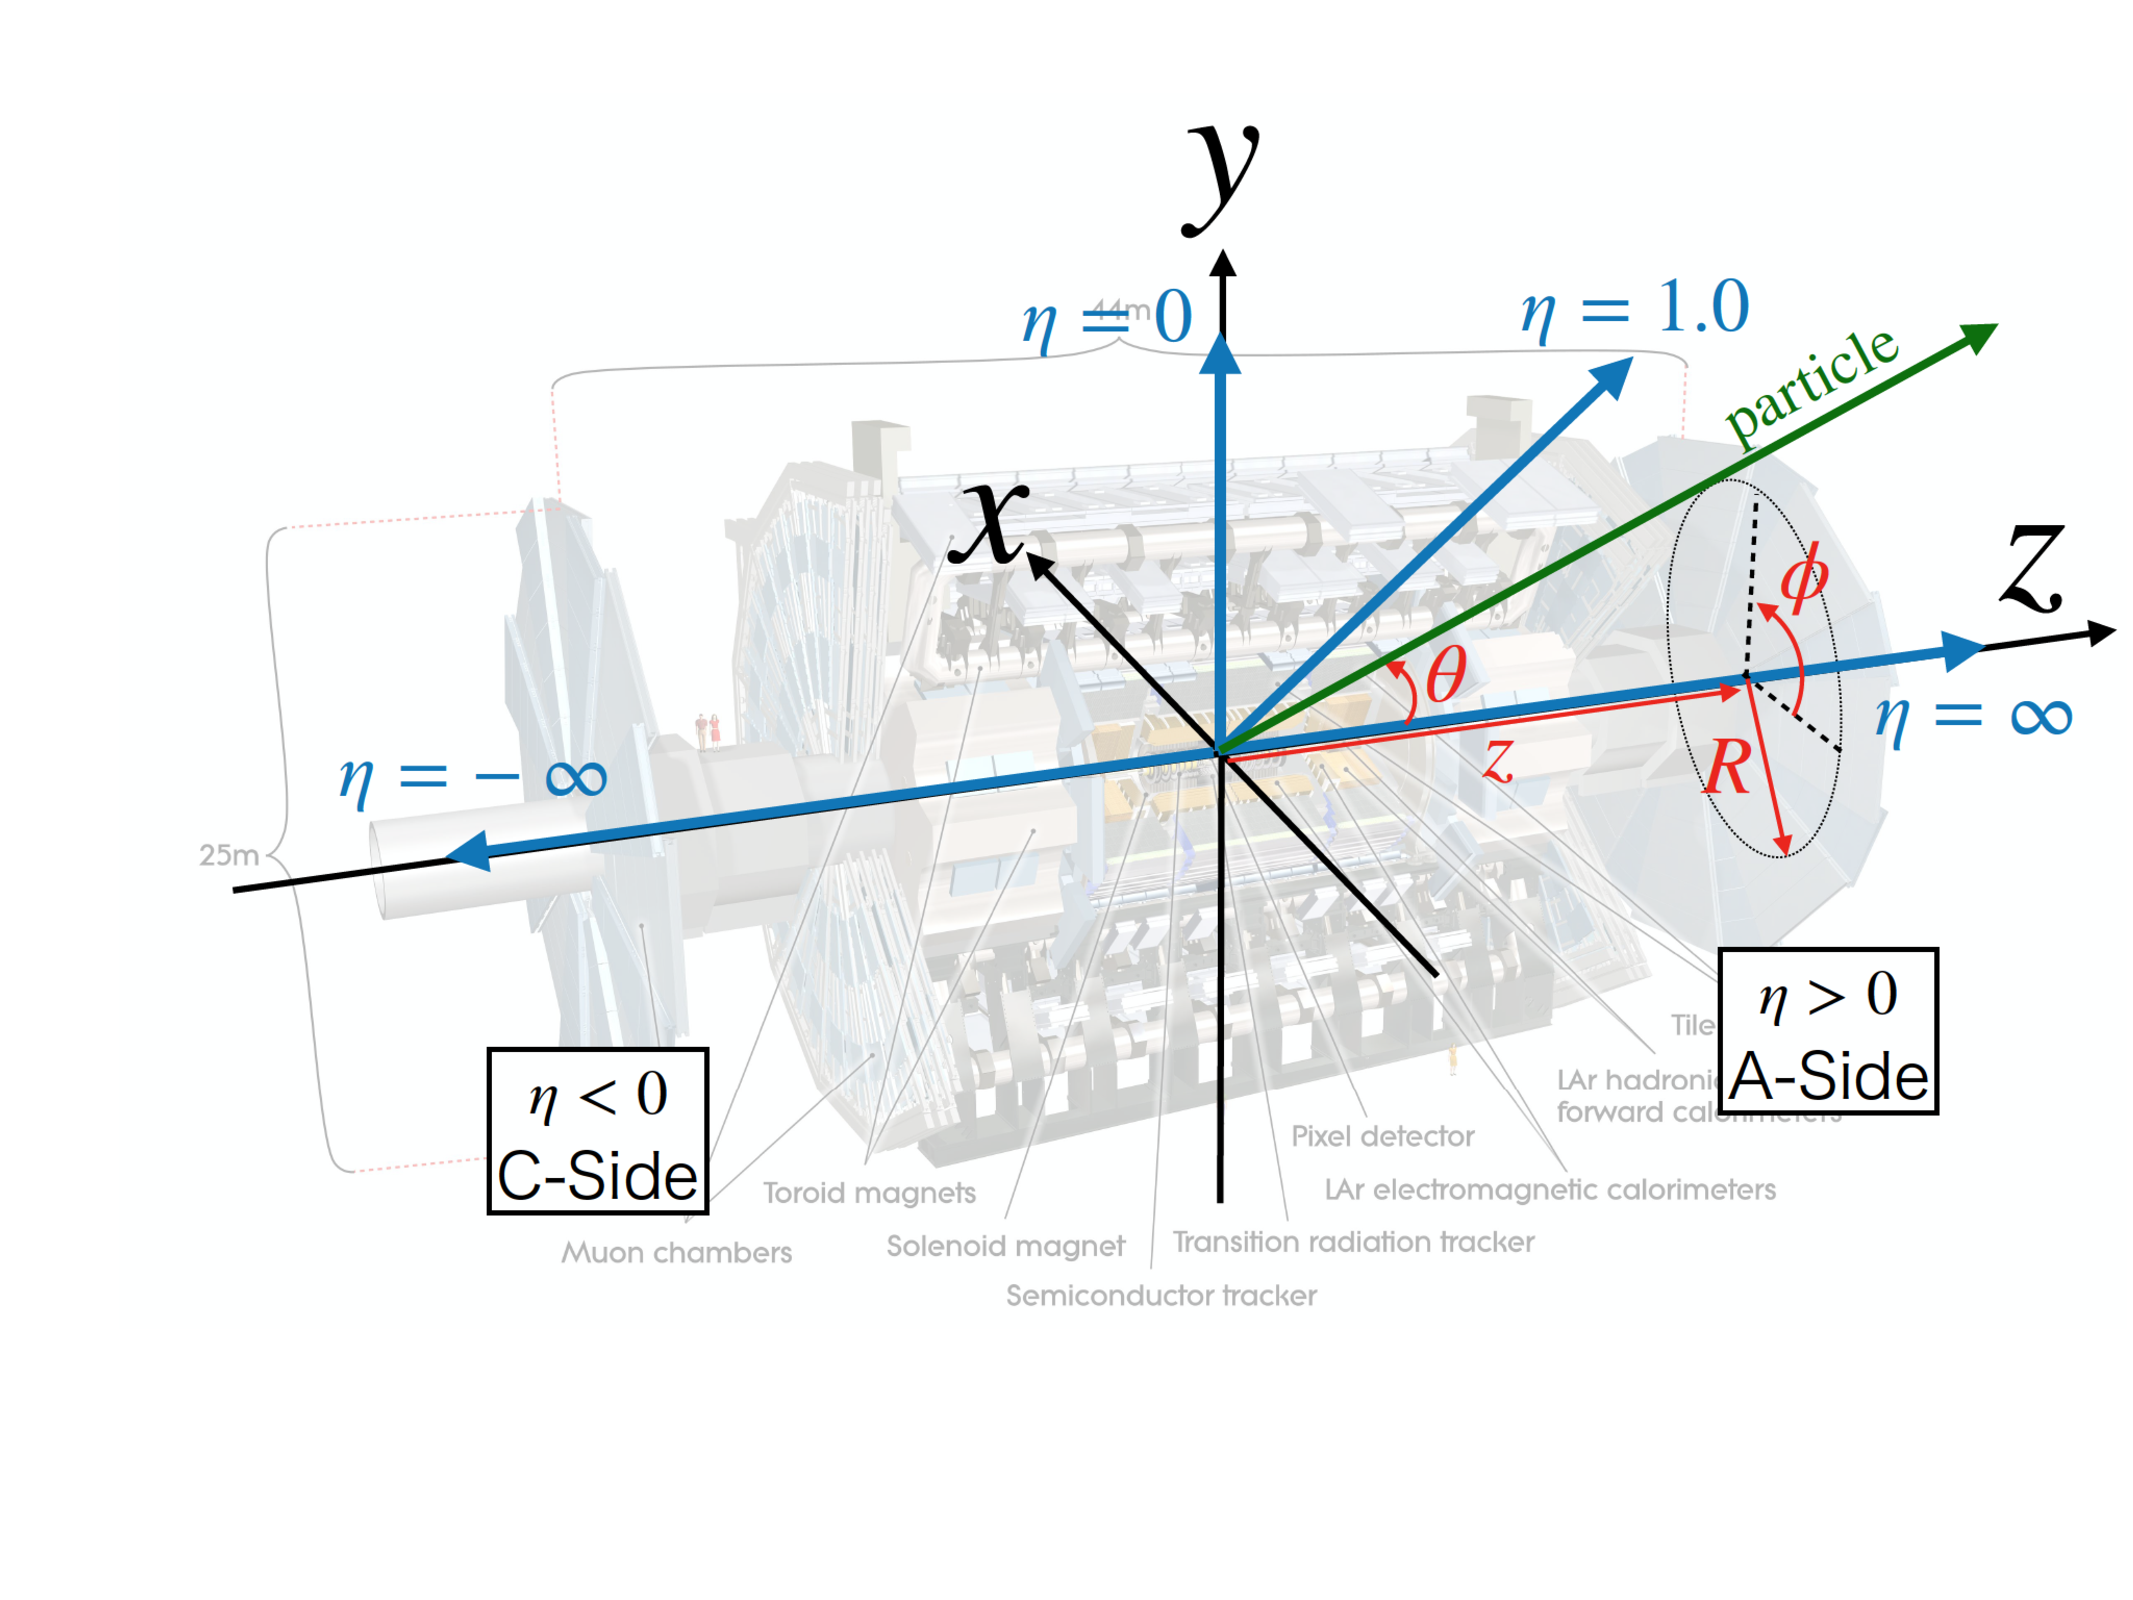
\includegraphics[width=\textwidth,page=1]{img/pdf/cood.pdf}
    \caption[ATLAS~実験において使用される座標系]{ATLAS~実験において使用される座標系。$x,~y,~z$方向に設定される直交座標系と$R,~\phi,~\theta$で定義される極座標系がある。$\theta$方向を表す量として、擬ラピディティ$\eta$が利用される。$\eta>0$を~A-Side、$\eta<0$を~C-Side~と呼ぶ。}\label{fig:cood}
\end{figure}

\subsection{超伝導マグネット}
ATLAS~におけるマグネットシステムは~3~種類の巨大な超電導磁石により構成されている。\figref{fig:mag}にATLAS検出器における超伝導マグネットの構成を示す。一つは中央のソレノイド磁石であり内部検出器の運動量測定に用いられる。流れる電流は~7.73~kA~で、ピーク磁場は~2.6~T~である。その周りを囲むバレル領域のトロイド磁石は、八回対称のリングで構成されており、円周方向の磁場を生成する。流れる電流は~20.5~kA~で、ピーク磁場は~3.9~T~である。エンドキャップ領域のトロイド磁石も同様に円周方向の磁場を生成する。流れる電流は~20.5~kA~で、ピーク磁場は約~4.1~T~である。これらのトロイド磁石はミューオンの運動量を測定するために利用されている。

\figref{fig:mag}に示すように、トロイド磁場の強さは一様ではなく基本的にコイルの配置と同様に八回対称になる。$0<|\eta|<1.4$における磁場の強さは約$1.5\sim5.5~\rm{Tm}$、$1.6<|\eta|<2.7$における磁場の強さは約$1\sim7.5~\rm{Tm}$となる。
磁場の弱い領域においては低い横運動量を持つミューオンと高い横運動量を持つミューオンの曲率の差がなくなり正確な横運動量測定ができなくなる。したがって初段ミューオントリガーにおいては、磁場の弱い領域で正しく運動量判定ができなかった事象を取り除くアルゴリズムが実装されている~(RoI~Mask)。
\begin{figure}[tbp]
        \begin{minipage}{0.49\hsize}
        \centering   
        \includegraphics[width=0.75\textwidth,page=5]{img/pdf/ATLAS.pdf}
        \subcaption{}
        \end{minipage}
        \begin{minipage}{0.49\hsize}
	    \centering
	    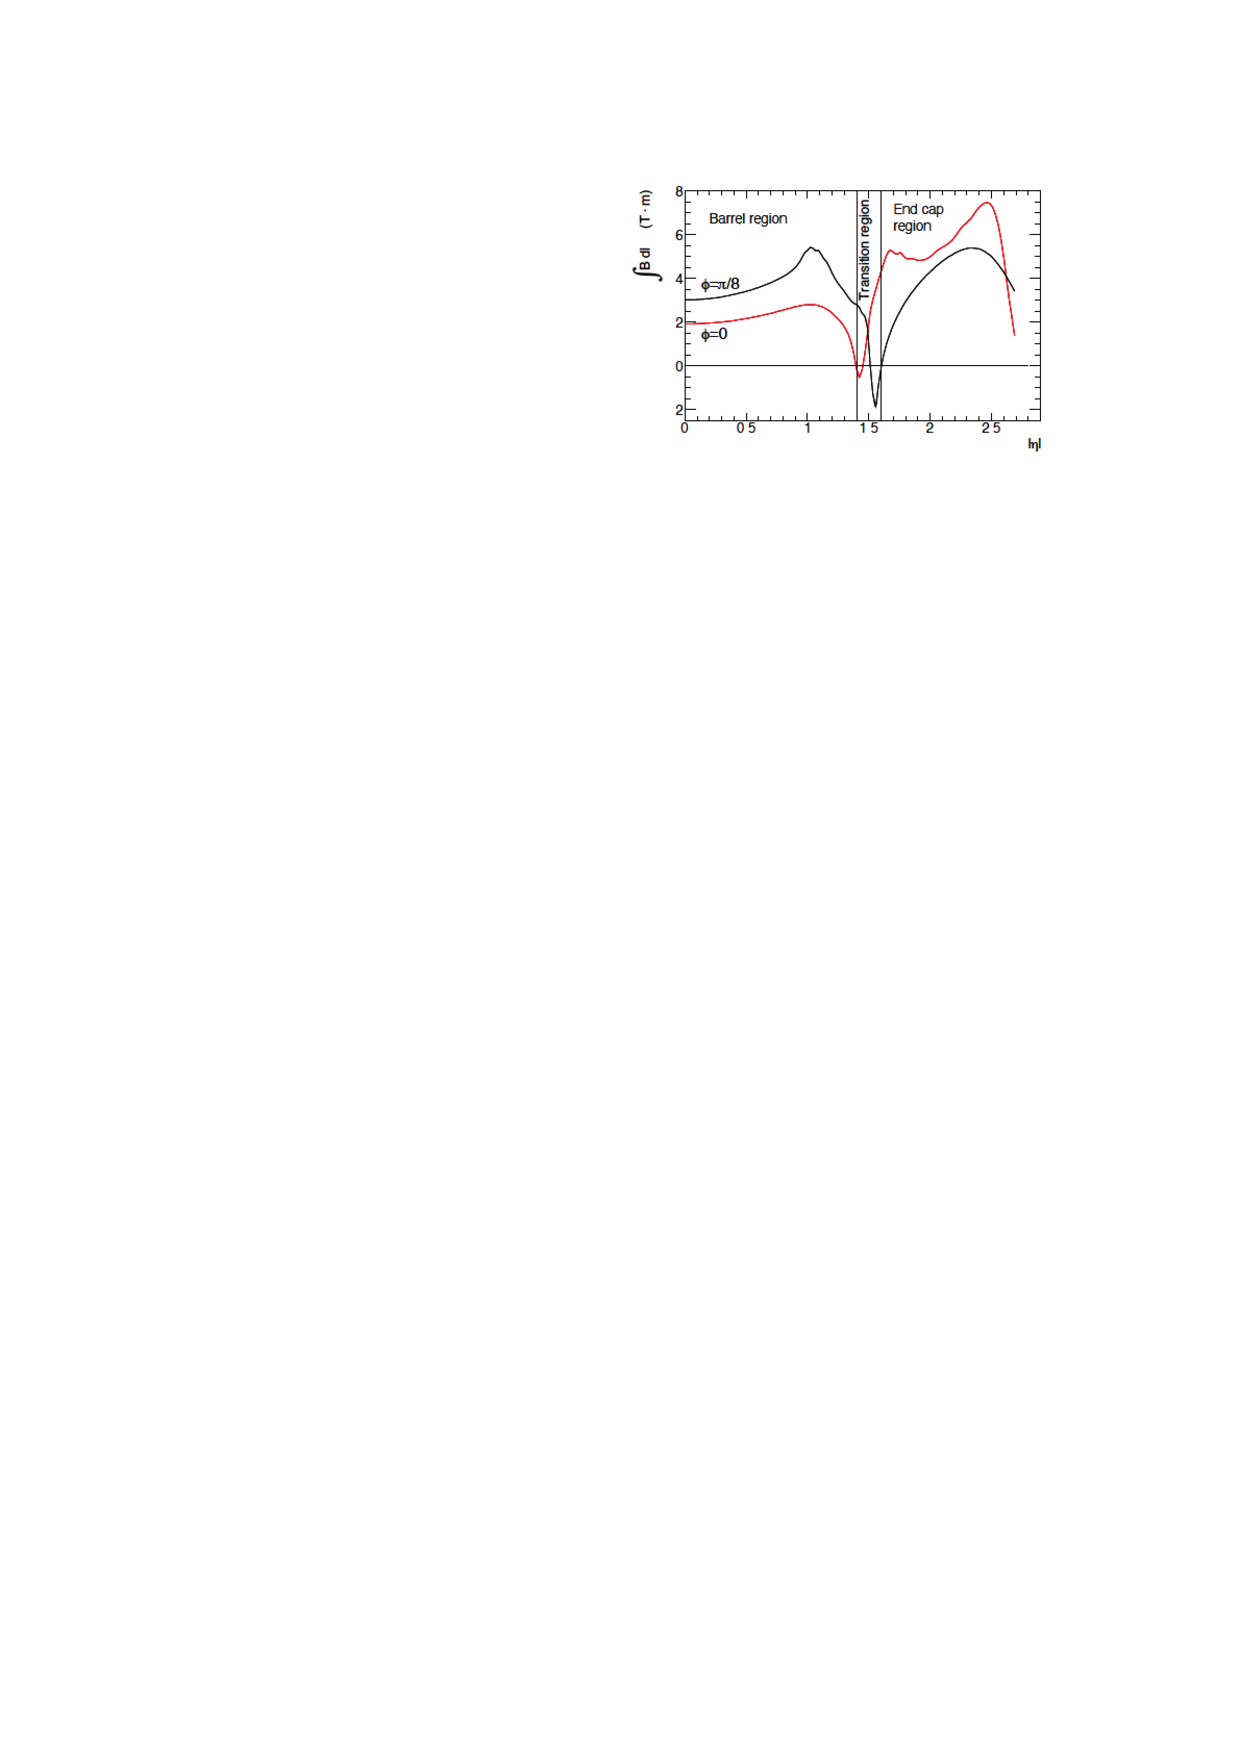
\includegraphics[width=\textwidth,page=1]{img/pdf/mag.pdf}
	    \subcaption{}
	    \end{minipage}
        \caption[ATLAS~検出器における超伝導磁石の構成とトロイド磁石による磁場の分布]{(a)ATLAS検出器における超伝導磁石の構成~\cite{TR:01}。衝突点付近のソレノイド磁石と外側のトロイド磁石で構成されている。トロイド磁場はエンドキャップ領域、バレル領域それぞれにおいて八回対称になるように設定されている。(b)~トロイド磁石による磁場の分布~\cite{TR:01}。無限運動量ミューオンに対するトロイダル磁石の予想磁場積分値を$|\eta|$の関数として表している。}\label{fig:mag}
\end{figure}

\subsection{内部飛跡検出器}
内部飛跡検出器~\cite{URL:19}はビーム衝突点に最も近い位置に設置され、ソレノイド磁石の内部に位置している。内側から順に、ピクセル検出器~(Pixel)、シリコントラッカー~(SCT)、遷移輻射トラッカー~(TRT)~の~3~つで構成されている。
~Pixel~は、最内層にある半導体検出器であり、高い位置分解能を持つ。SCT~はマイクロストリップと呼ばれる細長い有感領域をシリコン上に施した半導体検出器である。そして~TRT~は半径~4~mm~のチューブ型検出器であり、トラッキングのほかに遷移輻射を利用した電子の同定も行っている。
以上の内部飛跡検出器は、いずれもビーム衝突点に近く非常に厳しい放射線環境下にさらされるため、高い放射線耐性が必要不可欠である。\figref{fig:innr}に内部飛跡検出器の概略を示す。

\begin{figure}[tbp]
    \centering   
    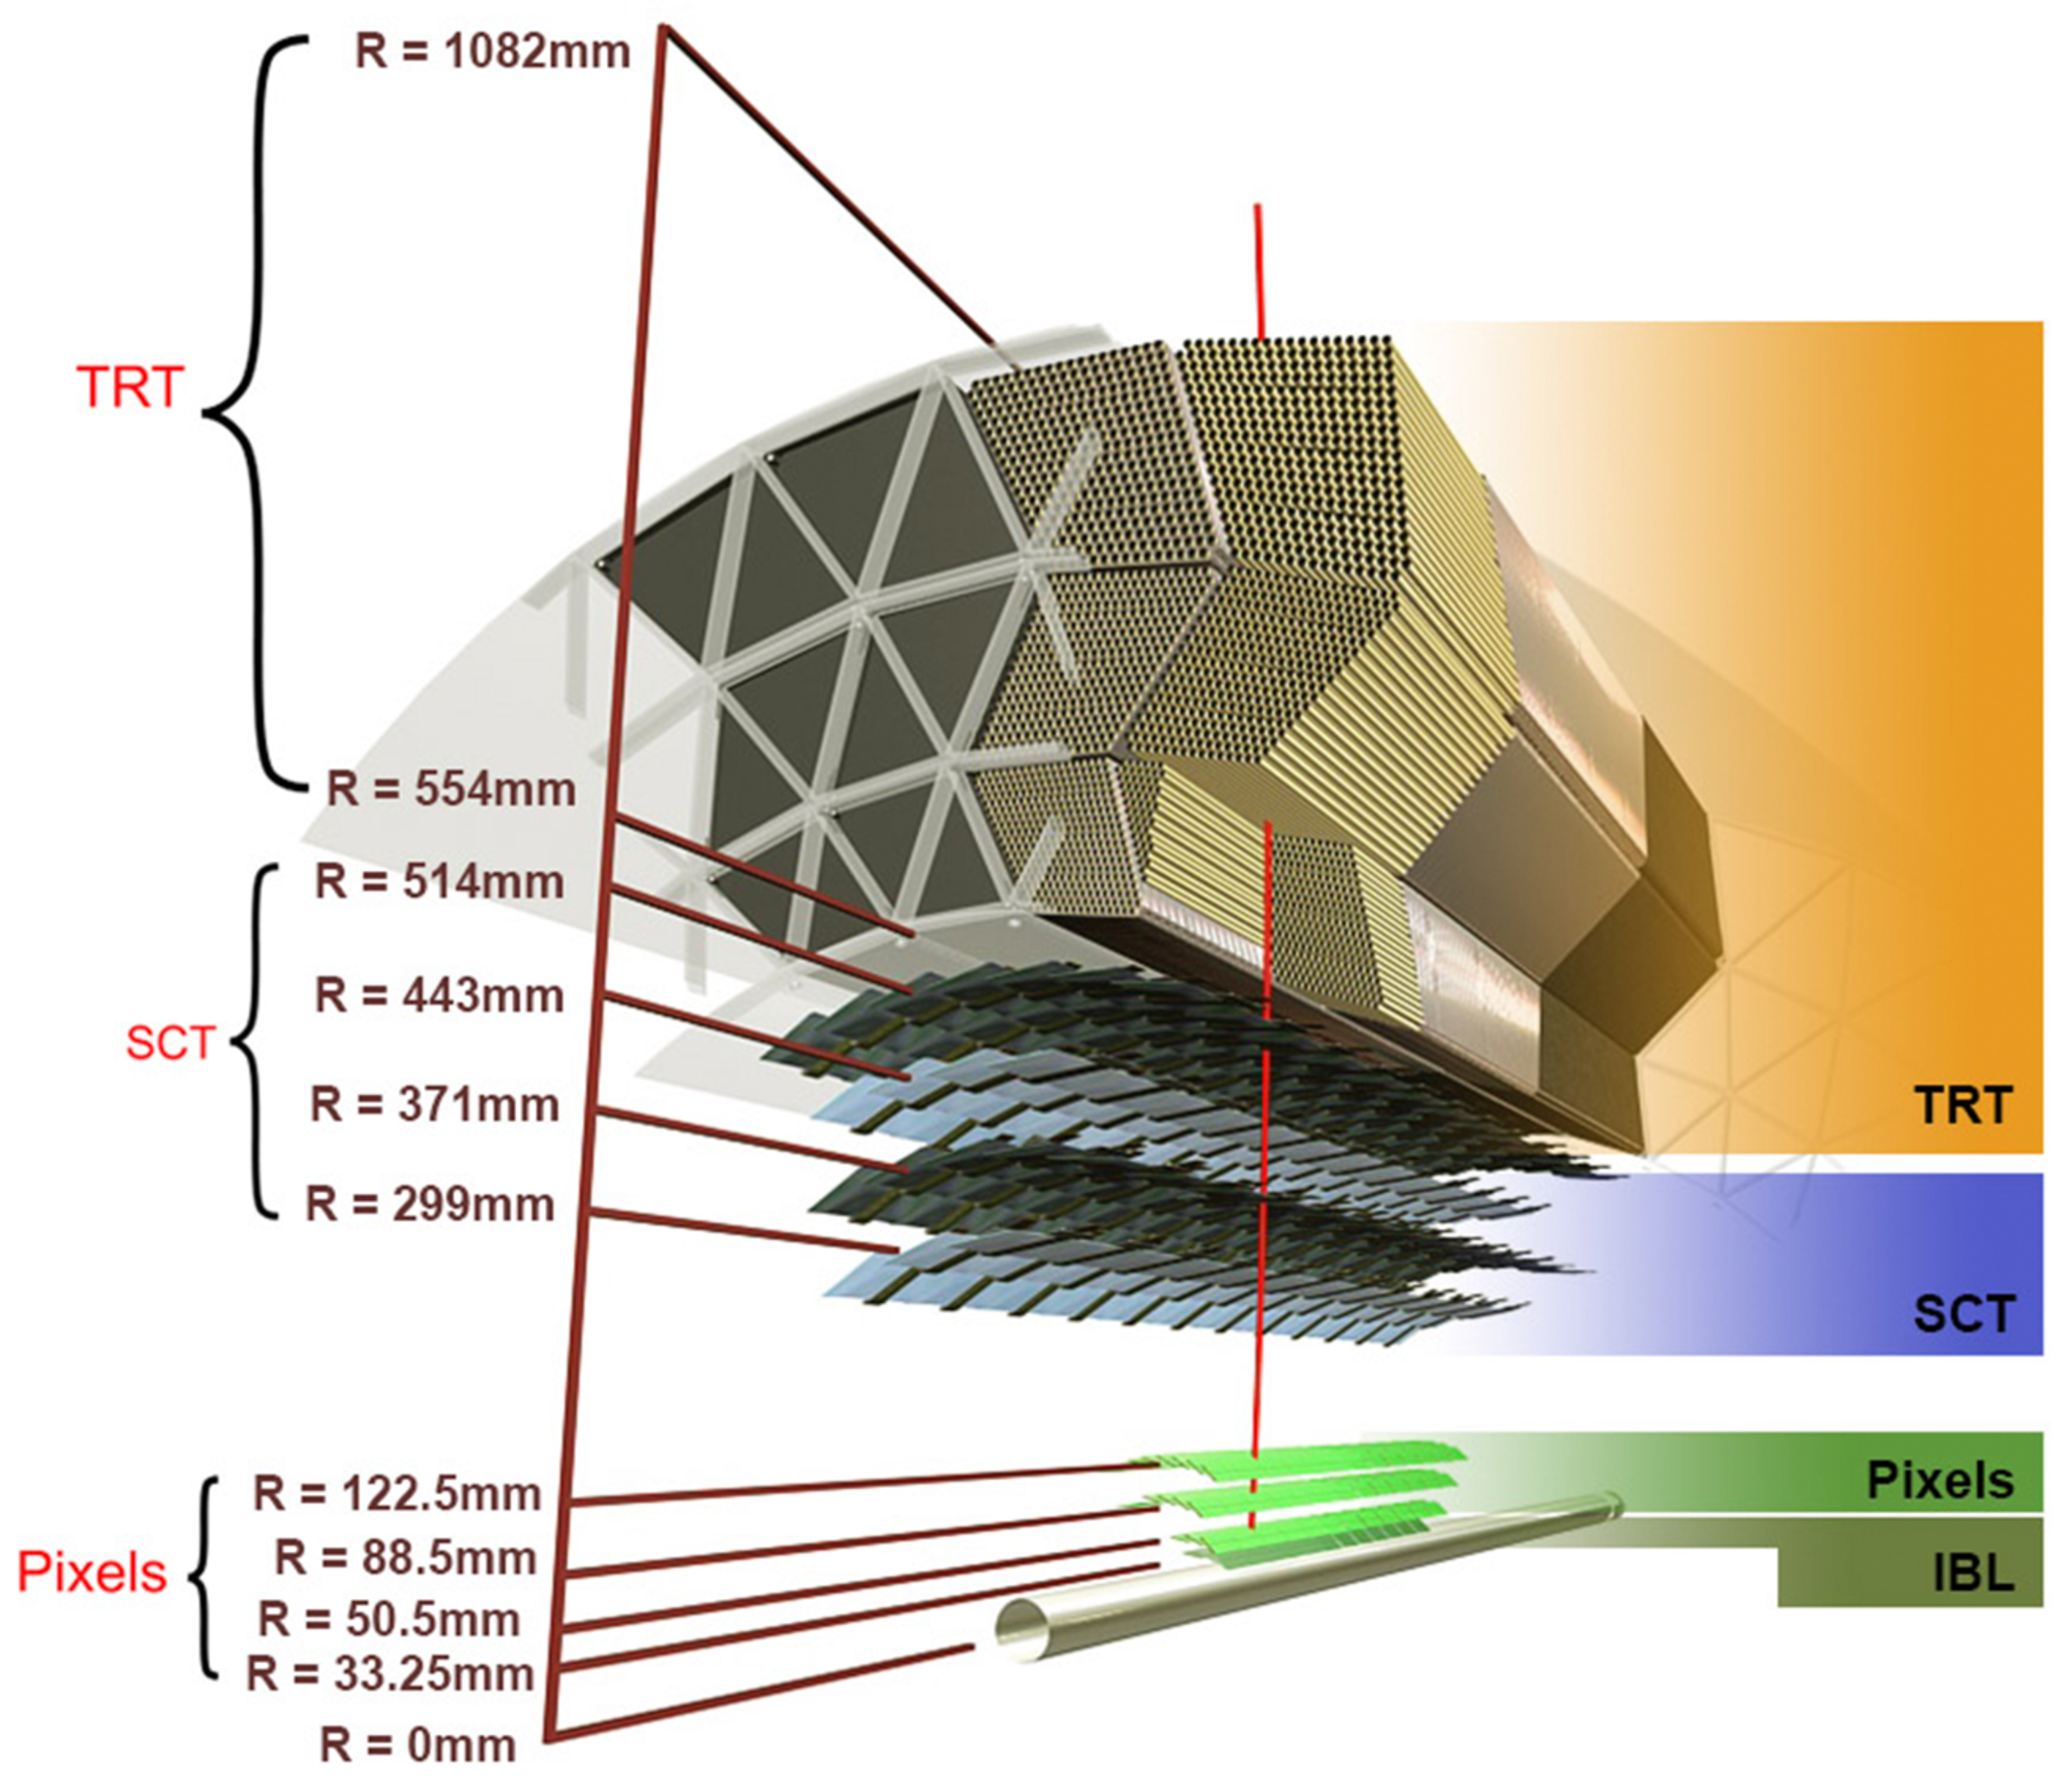
\includegraphics[width=0.8\textwidth,page=1]{img/jpeg/id.pdf}
    \caption[ATLAS~検出器における内部飛跡検出器の構成]{ATLAS~検出器における内部飛跡検出器の構成~\cite{URL:19}。内側から順に~Pixel,~SCT,~TRT~検出器が設置されている。}\label{fig:innr}
\end{figure}

\subsection{カロリメータ}
カロリメータの主な役割は、電子やガンマ線、ジェット等のエネルギーおよび角度の測定である。ATLAS~実験に使用される~4~種類のカロリメータは、電磁カロリメータとハドロンカロリメータの~2~つのいずれかに区分され、広範囲をカバーしている。\figref{fig:calo}にカロリメータの構成を示す。
以下では、それぞれのカロリメータについて簡単に説明する。

\begin{figure}[tbp]
        \centering   
        \includegraphics[width=0.8\textwidth,page=3]{img/pdf/ATLAS.pdf}
        \caption[ATLAS~検出器におけるカロリメータの構成]{ATLAS~検出器におけるカロリメータの構成~\cite{TR:01}。電磁カロリメータは、バレル領域およびエンドキャップ領域の~2~種類。ハドロンカロリメータは、バレル領域のタイル、エンドキャップ領域、フォワード領域の液体アルゴンカロリメータの~3~種類。}\label{fig:calo}
\end{figure}

\subsubsection{電磁カロリメータ}
電磁カロリメータは、アコーディオン構造のからなる鉛の吸収体と液体アルゴンで構成される。放射線耐性に優れており、電子と光子の同定に使用されている。ソレノイド磁石の外側に設置され、バレル領域$\cdot$エンドキャップ領域それぞれをカバーしている。

\subsubsection{ハドロンカロリメータ}
バレル領域では、鉄の吸収体とタイル状のシンチレータから構成されたタイルカロリメータが用いられている。放射線強度がより高いエンドキャップ領域では、銅の吸収体と液体アルゴンから構成されたカロリメータが使用されている。またさらに放射線強度の高いフォワード領域には、銅とタングステンの吸収体と液体アルゴンからなるカロリメータが設置されている。
以上のハドロンカロリメータは、電磁カロリメータの外側に設置されており、ハドロンの同定、エネルギー測定およびジェットの再構成を行う。


\subsection{ミューオン検出器}
終状態に荷電レプトンを含む事象は、ジェットを引き起こすハドロンなどに比べ、飛跡を再構成しやすく、測定装置で捕えやすい。特にミューオンは物質に対する透過力が高く、寿命が長いためにATLAS検出器の外側でもほかの検出器の影響を受けることなく検出することが可能である。ミューオン検出器は、飛跡の精密測定用の~Monitored~Drift~Tube~(MDT)、Cathorde~Strip~Chamber~(CSC)~と、トリガー用の~Resistive~Plate~Chamber~(RPC)、Thin~Gap~Chamber~(TGC)の~4~種類で構成され、ATLAS~検出器の最外層に設置されている検出器である。\figref{fig:mud}に各ミューオン検出器の構成を示す。
\begin{figure}[tbp]
        \centering   
        \includegraphics[width=0.7\textwidth,page=4]{img/pdf/ATLAS.pdf}
        \caption[ATLAS~検出器におけるミューオン検出器の構成]{ATLAS~検出器におけるミューオン検出器の構成~\cite{TR:01}。トリガー用の~RPC,~TGC~と精密測定用の~MDT,~CSC~で構成されている。}\label{fig:mud}
\end{figure}

MDT~はバレル領域とエンドキャップ領域の両方に設置され、直径~30~mm~のドリフトチューブによって構成されている。CSC~はフォワード領域の内側に設置されたストリップチェンバーである。 また~RPC~はバレル領域、TGC~はエンドキャップ領域をカバーするように配置されており、PRC~は~平行平板ガス検出器、TGC~は薄いギャップの~Multi~Wire~Proportional~Chamber~(MWPC)~である。ミューオン検出器の特徴の詳細に関しては、\tbref{tb:muon}に記す。
\begin{table}[tbp]
	\centering
	\begin{tabular}{c|ccc}\hline
	    検出器 & 役割 & カバー領域 & チャンネル数 \\ \hline\hline
		MDT & 運動量測定 & $0<|\eta|<3.0$ & 約370,000 \\ 
		CSC & 運動量測定 & $2.0<|\eta|<3.0$ & 約67,000 \\
        RPC & トリガー & $0<|\eta|<1.05$ & 約350,000 \\
        TGC & トリガー & $1.05<|\eta|<2.04$ & 約320,000 \\ \hline 
	\end{tabular}
	\caption{各ミューオン検出器における役割や特徴の一覧}
    \label{tb:muon}
\end{table}

バレル領域においてミューオン検出器は、大きく分けて円筒型の側面部~3~箇所に配置されている。またエンドキャップ領域では円筒型の底面部~3~箇所に配置されている。バレル・エンドキャップそれぞれにビーム衝突点に近い方から、Inner,~Middle,~Outer~と呼んでいる。\figref{fig:tgc000}にATLAS検出器における断面図と~TGC~検出器の配置を示した。TGC~は、Middle~に~M1,~M2,~M3~の~3~ステーション、トロイドマグネット内側の~Inner~に~EIFI~ステーションの合計~4~ステーションで構成されている。TGC~検出器における構成やエレクトロニクスに関する詳細は\chapref{chap:4}で述べる。
\begin{figure}[tbp]
    \centering
    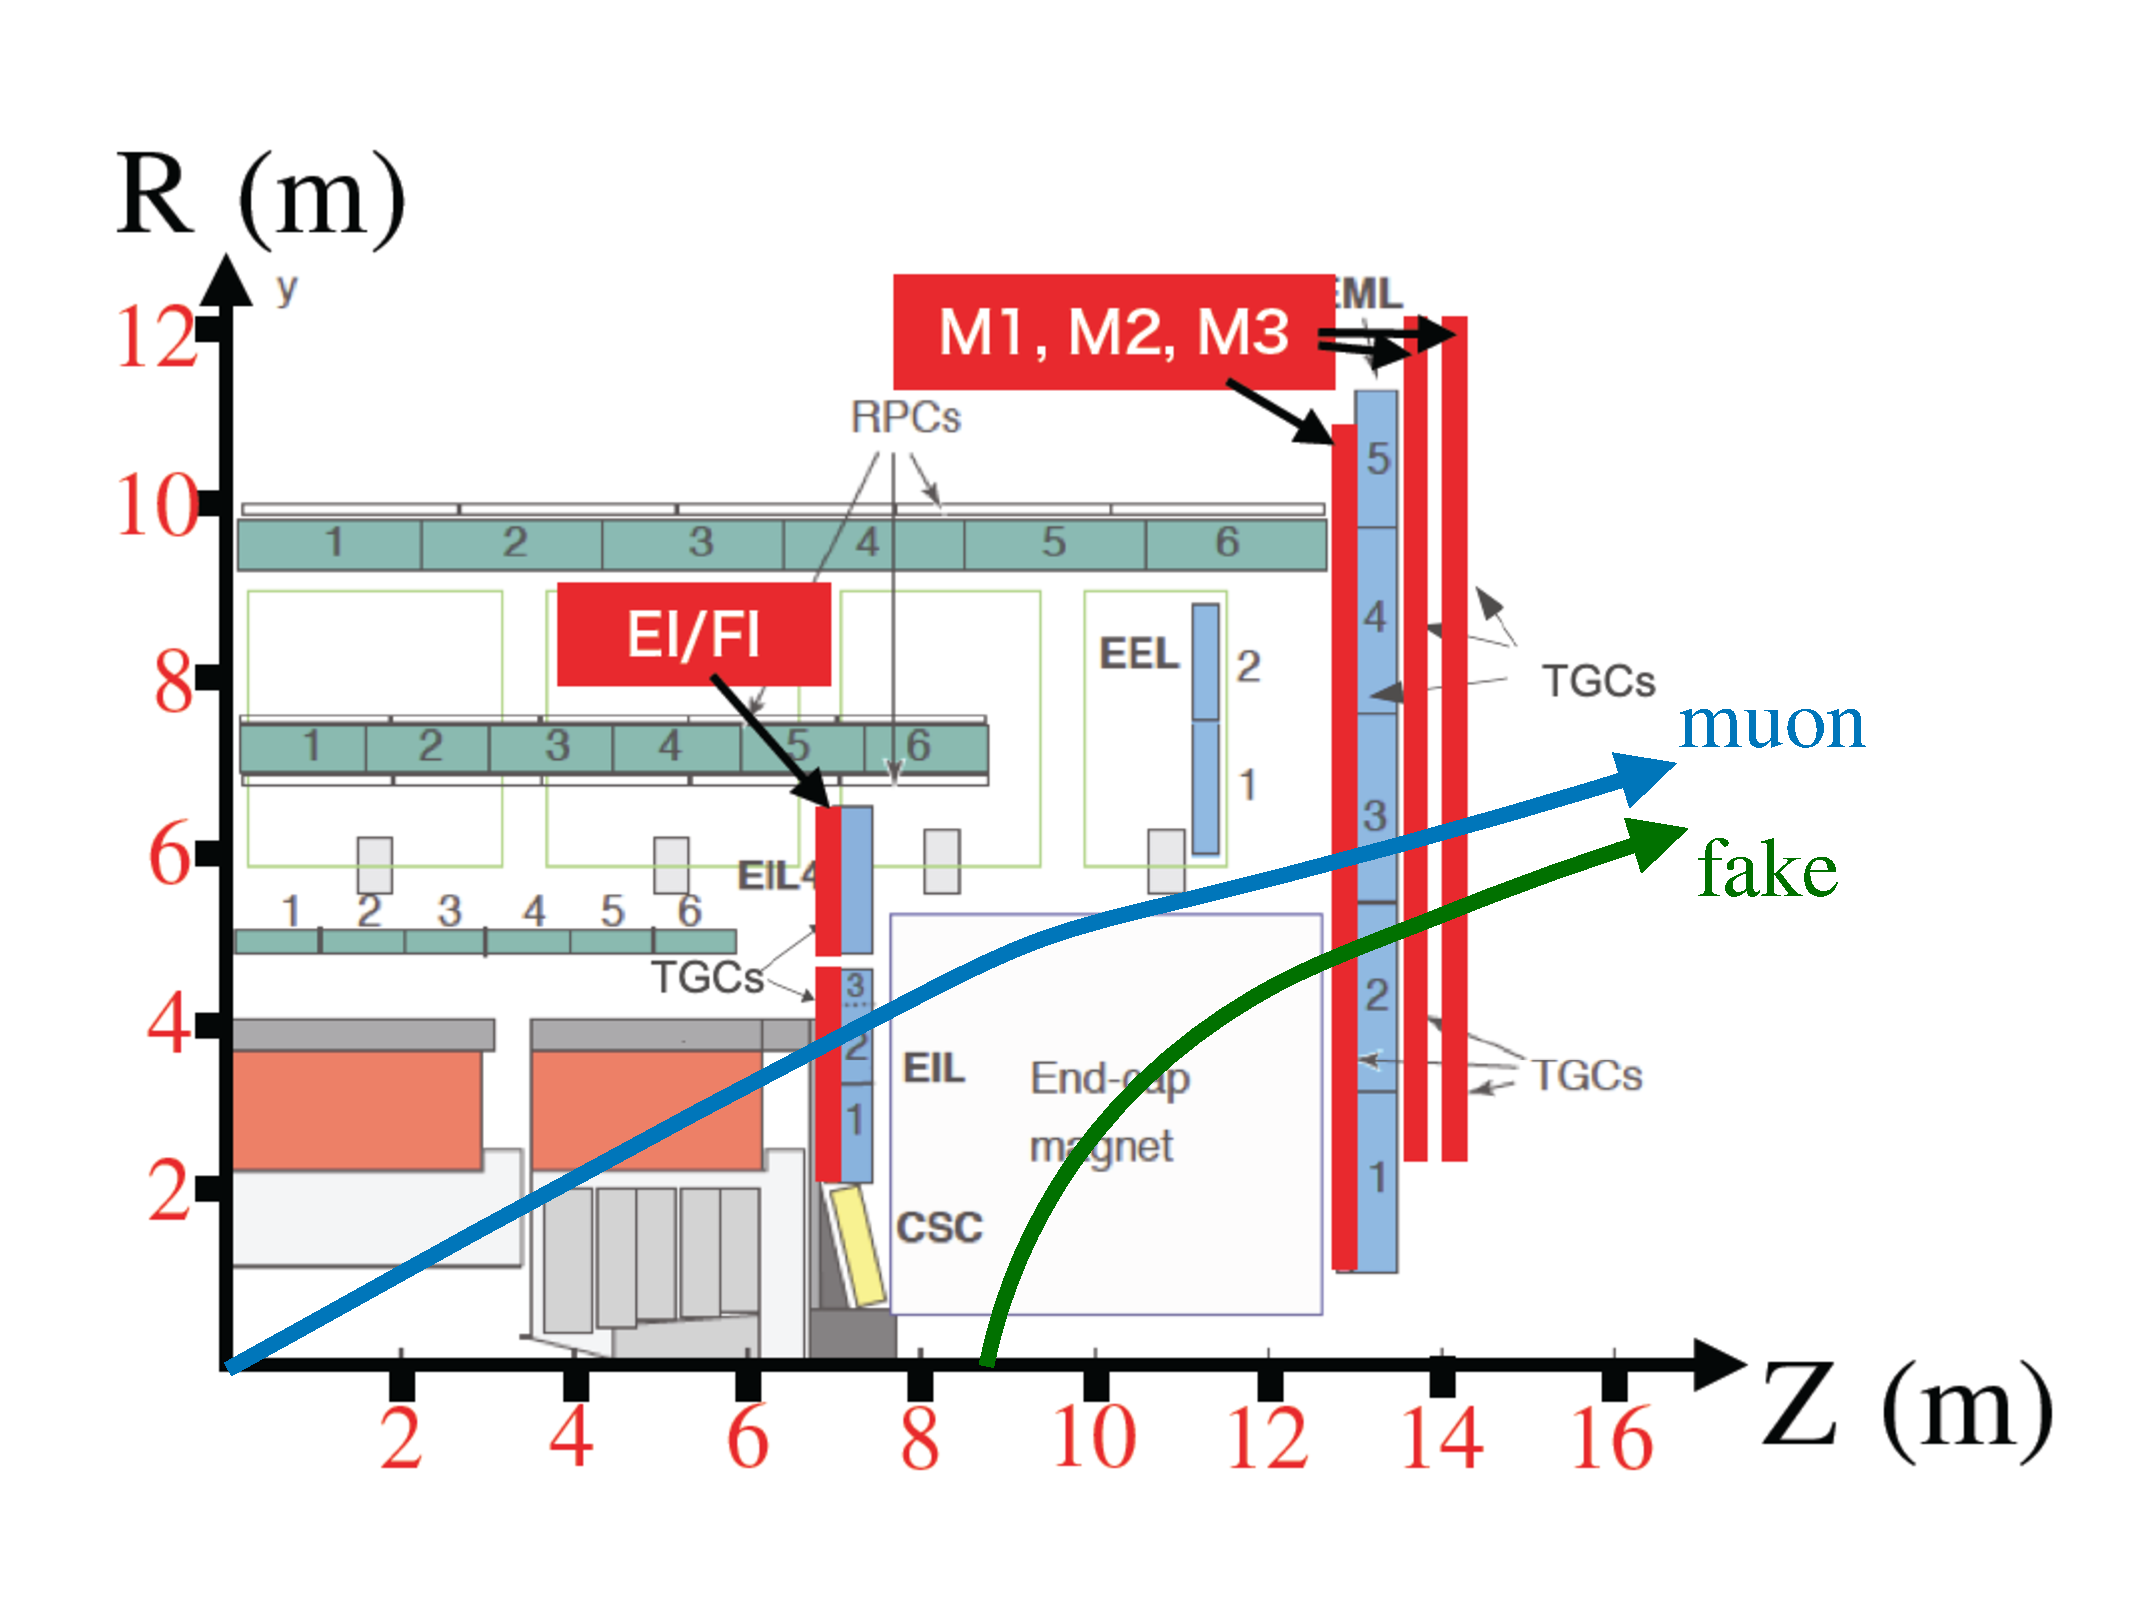
\includegraphics[width=0.8\textwidth,page=1]{img/pdf/fake.pdf}
    \caption[Run~2~におけるATLAS検出器を$R-z$方向から見たときの断面図および~TGC~各ステーションの配置]{Run~2~におけるATLAS検出器を$R-z$方向から見たときの断面図および~TGC~各ステーションの配置~\cite{TR:01}。Big~Wheel~は、M1~(3~層)、M2~(2~層)、M3~(2~層)の計~7~層で構成されており、Small~Wheel~は、EIFI~(2~層)~で構成されている。また青の矢印は衝突点で生成されたミューオンの飛跡、緑の矢印はビームパイプ由来の低速粒子の飛跡を示す。}\label{fig:tgc000}
\end{figure}

超電導トロイダル磁石は、バレル領域およびエンドキャップ領域にそれぞれ$\phi$方向の磁場を生成している。$\phi$方向の磁場によって$R-z$平面内で曲げられたミューオンの曲率を測定することで運動量を決定する。理想的にはミューオンは$R-z$平面内で曲がるが、実際は磁場の大きさが一様でないため$\phi$方向にも曲がる。トリガー用の~2~つの検出器~(RPC,~TGC)~は、$\phi$方向の座標を測る役割も担っている。

\subsubsection{Run~3~におけるミューオン検出器のアップグレード}
初段ミューオンエンドキャップトリガーでは、\figref{fig:tgc000}で示したようなビームパイプから発生した陽子などの低速粒子による影響が課題となっていた。これらの粒子が高い$p_{\rm{T}}$を持つミューオンと同じ角度で入射した場合、誤ってトリガーを発行してしまう。2012~年に取得した~Run~1~の解析結果によると、初段エンドキャップミューオントリガーで出力されたうちの約$90\%$がフェイクであった~\cite{TR:05}。その後の~Run~2~では、エンドキャップトロイドマグネットの内側に設置されたタイルカロリメータおよび~TGC~EIFI~とのコインシデンスを導入した。このようなインナーコインシデンスを要求することで、$1.05<|\eta|<1.7$の領域におけるフェイクトリガーの削減に成功している。

$1.92<|\eta|<2.4$の領域ではインナーコインシデンスを行うための検出器が設置されていないため、フェイクトリガーが多く残っており、$1.05<|\eta|<1.92$の領域においてもフェイク削減の余地は残っている。そこで~Run~3~においてはさらなるフェイクトリガーの削減を目指し、トロイド磁場領域の内側に~New~Small~Wheel~(NSW)~および~RPC~Barrel~Inner~Small~sector~78~(RPC~BIS78)~の~2~つの検出器を新たに導入する。\figref{fig:innercoin}に示すように、Run~3~では~2~つの検出器の導入でさらなるフェイクトリガーの削減が可能であることが見積もられている。Run~3~における~新検出器導入後のATLAS検出器の断面図を\figref{fig:cut3}に示す。
\begin{figure}[tbp]
        \centering   
        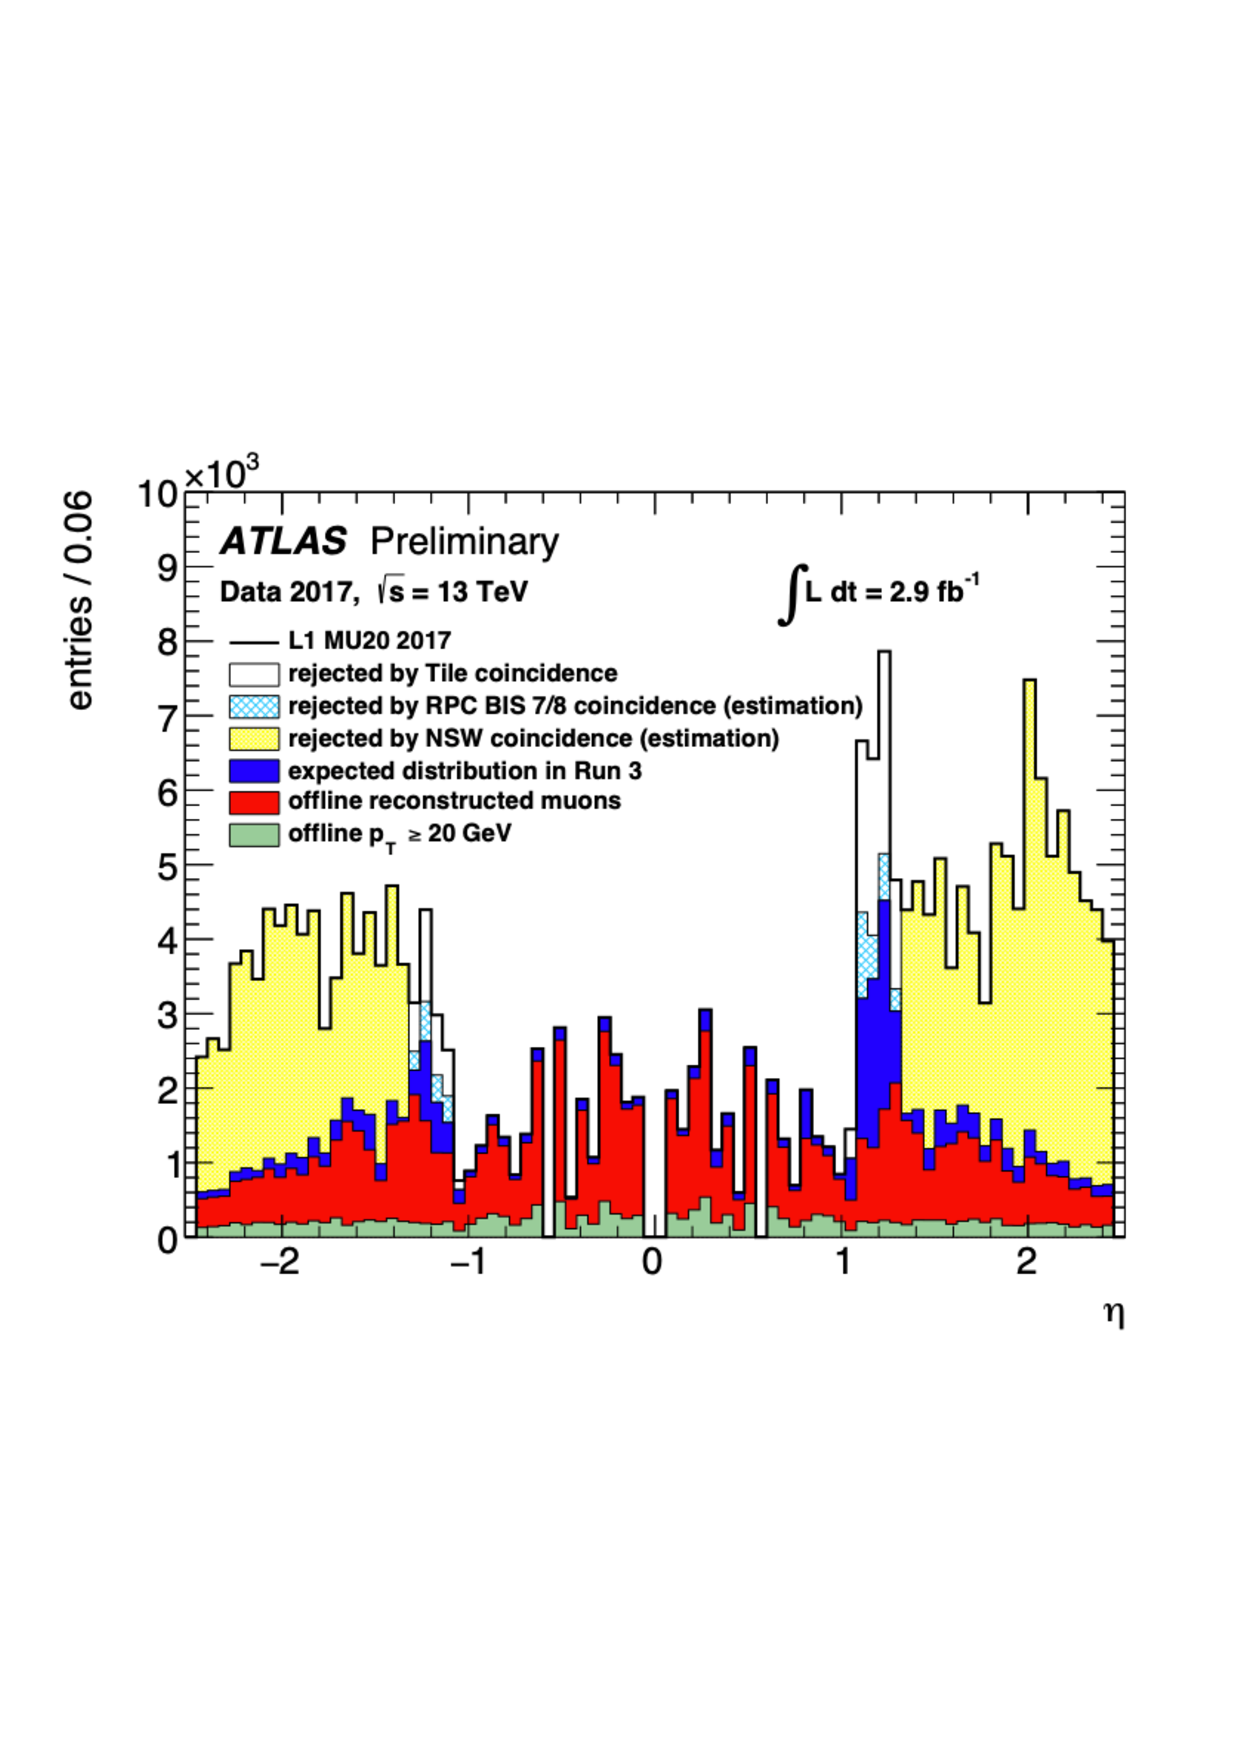
\includegraphics[width=0.7\textwidth,page=1]{img/pdf/inner.pdf}
        \caption[インナーコインシデンスによるフェイクトリガーの削減]{インナーコインシデンスによるフェイクトリガーの削減~\cite{shiomi}。Run~3~における初段ミューオントリガーを用いて選出したミューオン候補数の$\eta$分布の予測。タイル、RPC~BIS78~および~NSW~によって削減できるミューオン候補の数を示している。}
        \label{fig:innercoin}
\end{figure}
\begin{figure}[tbp]
        \centering   
        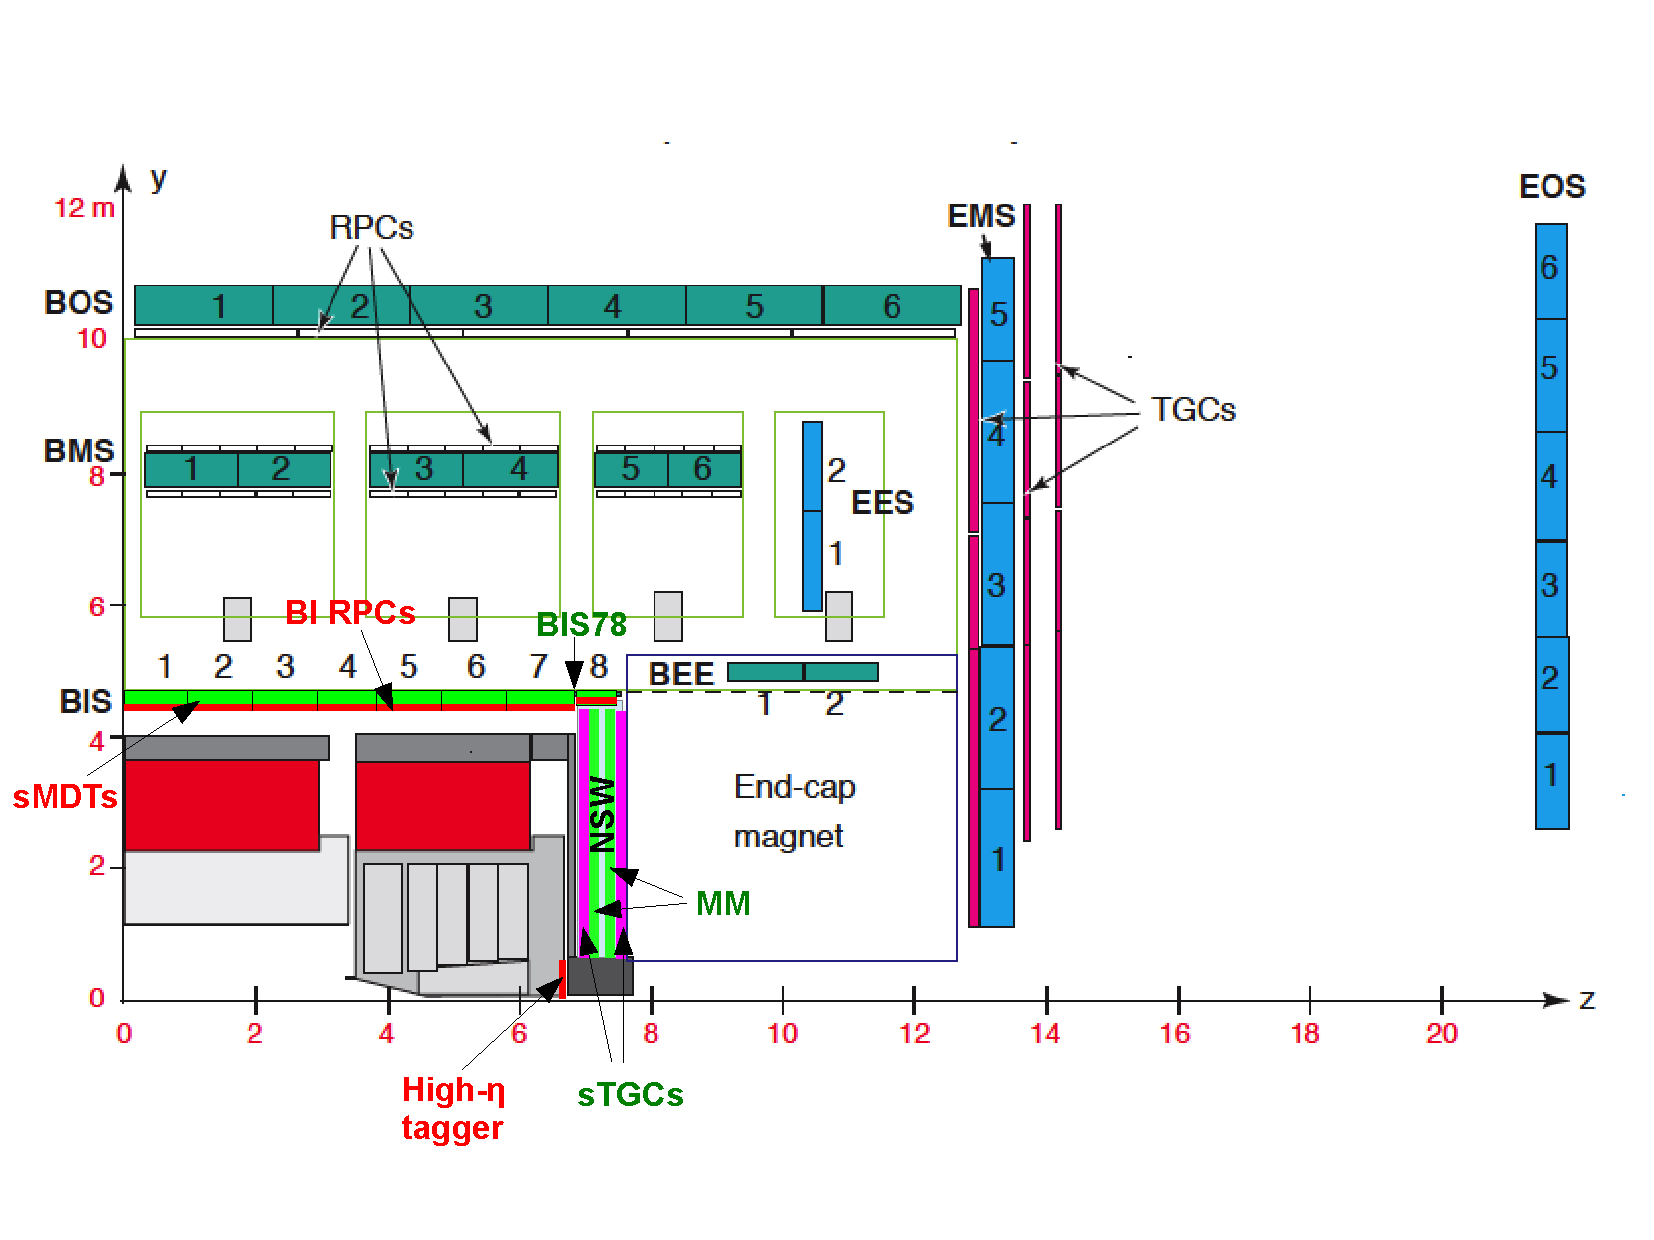
\includegraphics[width=0.8\textwidth,page=1]{img/pdf/ch01_fig_03a.pdf}
        \caption[NSW~および~RPC~BIS78~が導入された~Run~3~におけるATLAS検出器断面図]{NSW~および~RPC~BIS78~が導入された~Run~3~におけるATLAS検出器断面図~\cite{TR:04}。}
        \label{fig:cut3}
\end{figure}
\figref{fig:nsw}に~NSW~の構成を示す。
\begin{figure}[tbp]
    \begin{minipage}{0.49\hsize}
	\centering			
	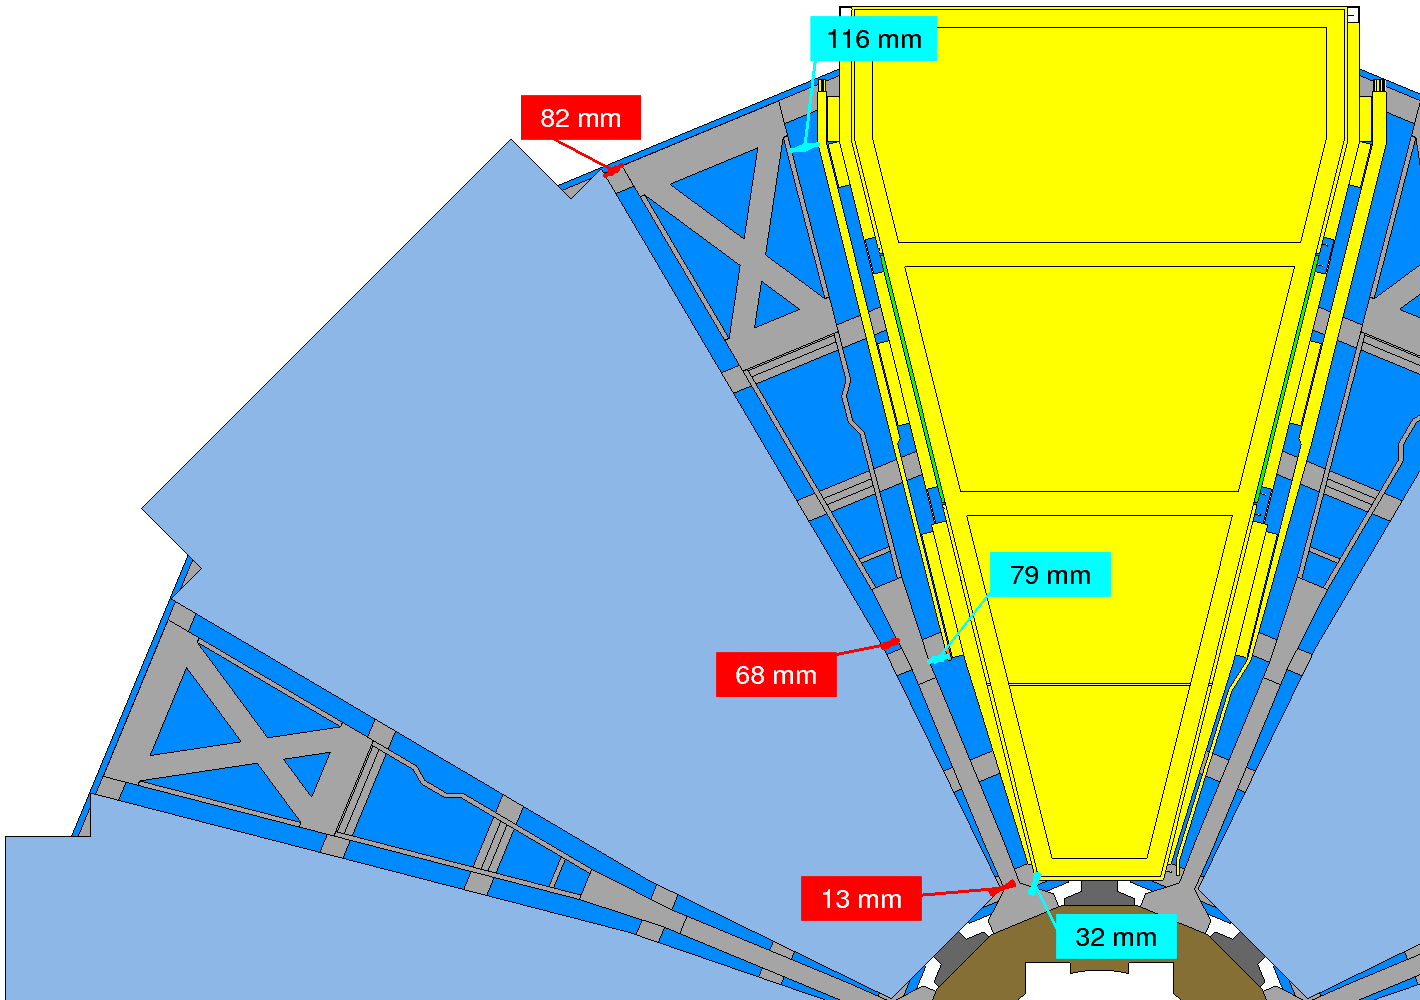
\includegraphics[width=\textwidth,page=1]{img/pdf/fig_026c.png}
	\subcaption{}
	\end{minipage}
	\begin{minipage}{0.49\hsize}
	\centering
	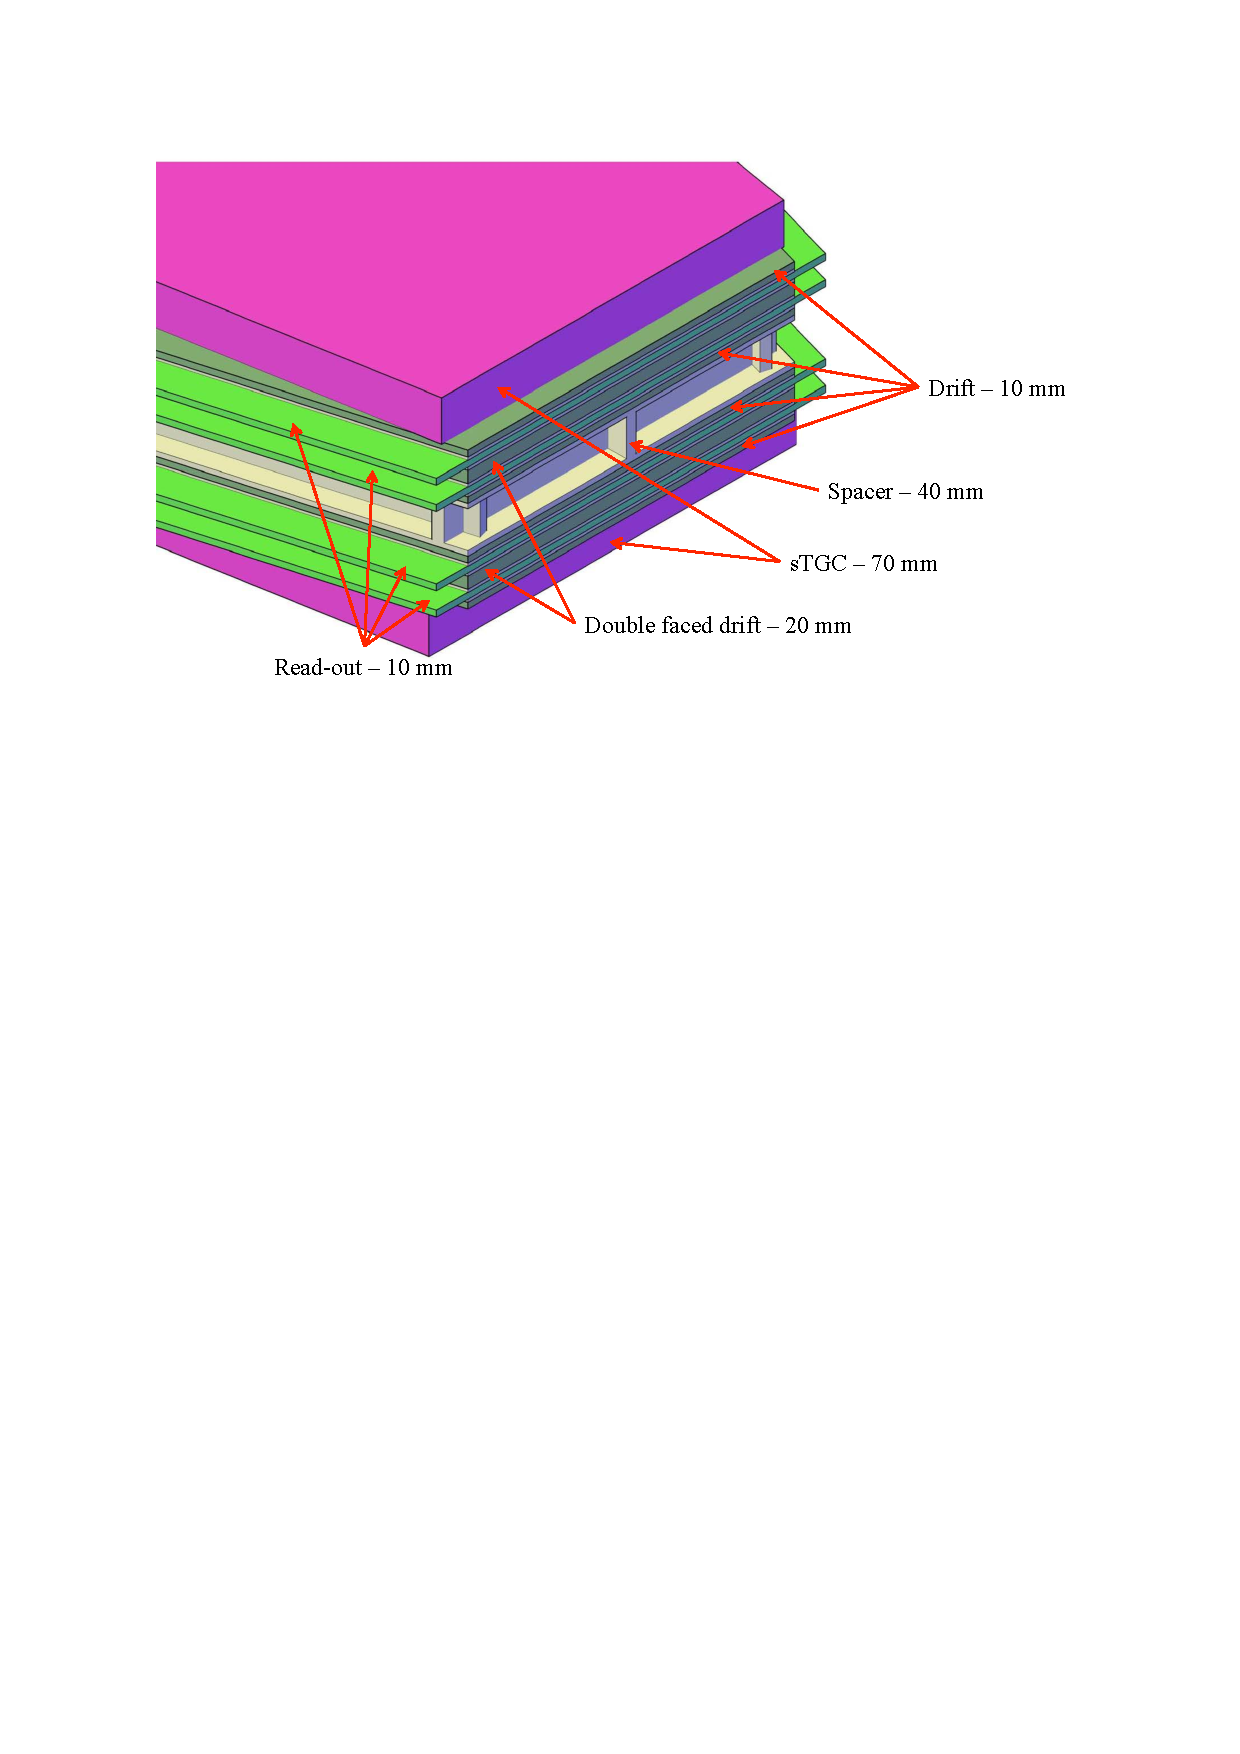
\includegraphics[width=\textwidth,page=1]{img/pdf/fig_042a.pdf}
	\subcaption{}
	\end{minipage}
    \caption[New~Small~Wheel~の構成]{New~Small~Wheel~の構成~\cite{AR:14}。4~層の~sTGC~の間に、4~層の~MM~が~2~台挟まれる構造となっている。(a)~チェンバーの全体図。(b)~NSW~の構成。}
    \label{fig:nsw}
\end{figure}
NSW~は$1.3<|\eta|<2.7$の領域をカバーするガス検出器である。NSW~は、Run~2~で使用されていた~TGC~FI、MDT~EIL~チェンバー、CSC~と入れ替わる形で導入される。したがって、NSW~は~TGC~FI~が担っていたミューオントリガーの役割および~MDT~と~CSC~が担っていた飛跡の精密測定の役割を果たすこととなる。そのため、NSW~は~small-strip~TGC~(sTGC)~と~Micromegas~(MM)~という二つの異なる技術の検出器で構成されている。NSW~を導入することでインナーコインシデンスの領域が$|\eta|<2.4$まで拡張される。

\figref{fig:bis}に~RPC~BIS78~の構成を示す。
\begin{figure}[tbp]
        \centering   
        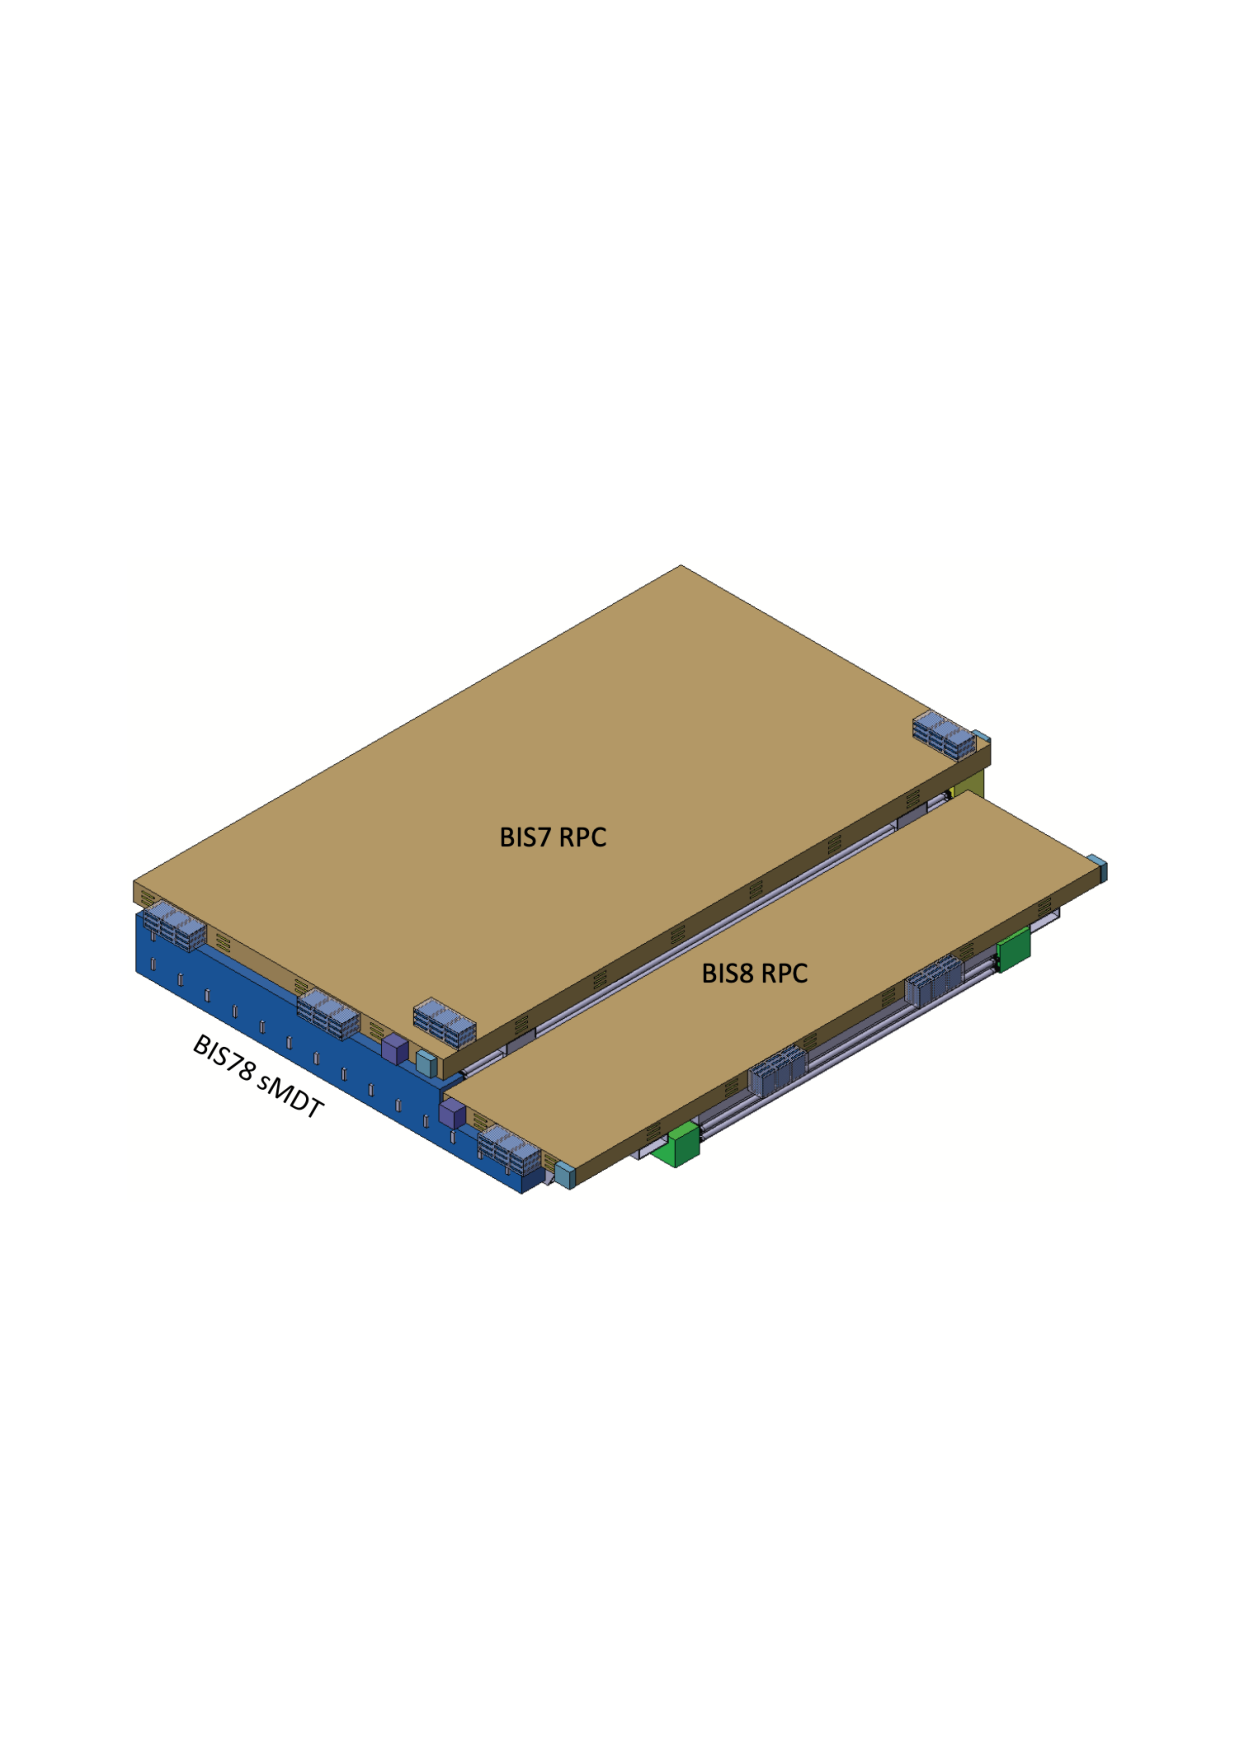
\includegraphics[width=0.8\textwidth,page=1]{img/pdf/bis.pdf}
        \caption[RPC~BIS78~の構成]{BIS78~の構成~\cite{TR:04}。RPC~および~sMDT~で構成される。}
        \label{fig:bis}
\end{figure}
Run~3~ではより高精度な測定を行うために~RPC~および~small-diameter~MDT~(sMDT)~を組み合わせた~RPC~BIS78~を新たに設置する。RPC~BIS78~は$1.0<|\eta|<1.3$の領域をカバーし、3~層のガス層で構成される。ガス層の厚みは約1~mmで、従来の~RPC~の半分になっている。ガス層は従来の~RPC~と同様に~2~次元方向のストリップで$\eta,~\phi$方向が測定できる。

\section{ATLAS~トリガーシステム}\label{sec:ttri}
LHC~での陽子陽子衝突から生成される粒子は~ATLAS~のトリガーシステムを介して選別される。
ATLAS~実験では、陽子がクォークとグルーオンとの複合粒子であることと高いルミノシティであることから、非常に高いイベントレートとなることが考えられる。トリガーシステムにおいては、物理解析のために必要な情報をいかに効率よく正確に選別できるかが鍵を握る。

ATLAS~実験の高頻度~(40~MHz)~陽子バンチ衝突に対して、最終的にデータとしての記録を許容できるイベントレートは数~kHz~である。この制限を満たし効率よくトリガーを行うために、ATLAS~実験ではハードウェアベースの初段トリガー~(Level-1~Trigger:~L1)~とソフトウェアベースの後段トリガー~(High-Level~Trigger:~HLT)~の二段階で実装されている。
\figref{fig:trigger}において、ATLAS 実験におけるトリガーと読み出し処理の流れについて示す。
本節では、ATLAS~実験におけるトリガーシステムについて詳しく説明する。
\begin{figure}[tbp]
        \centering   
            \includegraphics[width=\textwidth,page=2]{img/pdf/tdaq-run3-schematic-withoutFTK.pdf}
        \caption[Run~3~における~ATLAS~トリガーシステムの流れ]{Run~3~における~ATLAS~トリガーシステムの流れ~\cite{URL:07}。L1~では$2.5~\mu\rm{s}$以内にイベントレートを$100~\rm{kHz}$にまで削減する。L1~には~L1Calo,~L1Muon,~L1Topo~の~3~種類が存在する。HLT~ではソフトウェアベースでより詳細にトリガーを行い、数秒以内にイベントレートを数~kHz~にまで削減する。}\label{fig:trigger}
\end{figure}

\subsection{初段トリガー}\label{subsec:l1tri}
\subsubsection{初段トリガーでの処理の流れ}
初段トリガー~(L1)~におけるデータ処理の流れについて説明する。
\figref{fig:pipe}に~L1~における情報処理の流れを示す。
\begin{figure}[tbp]
        \centering   
        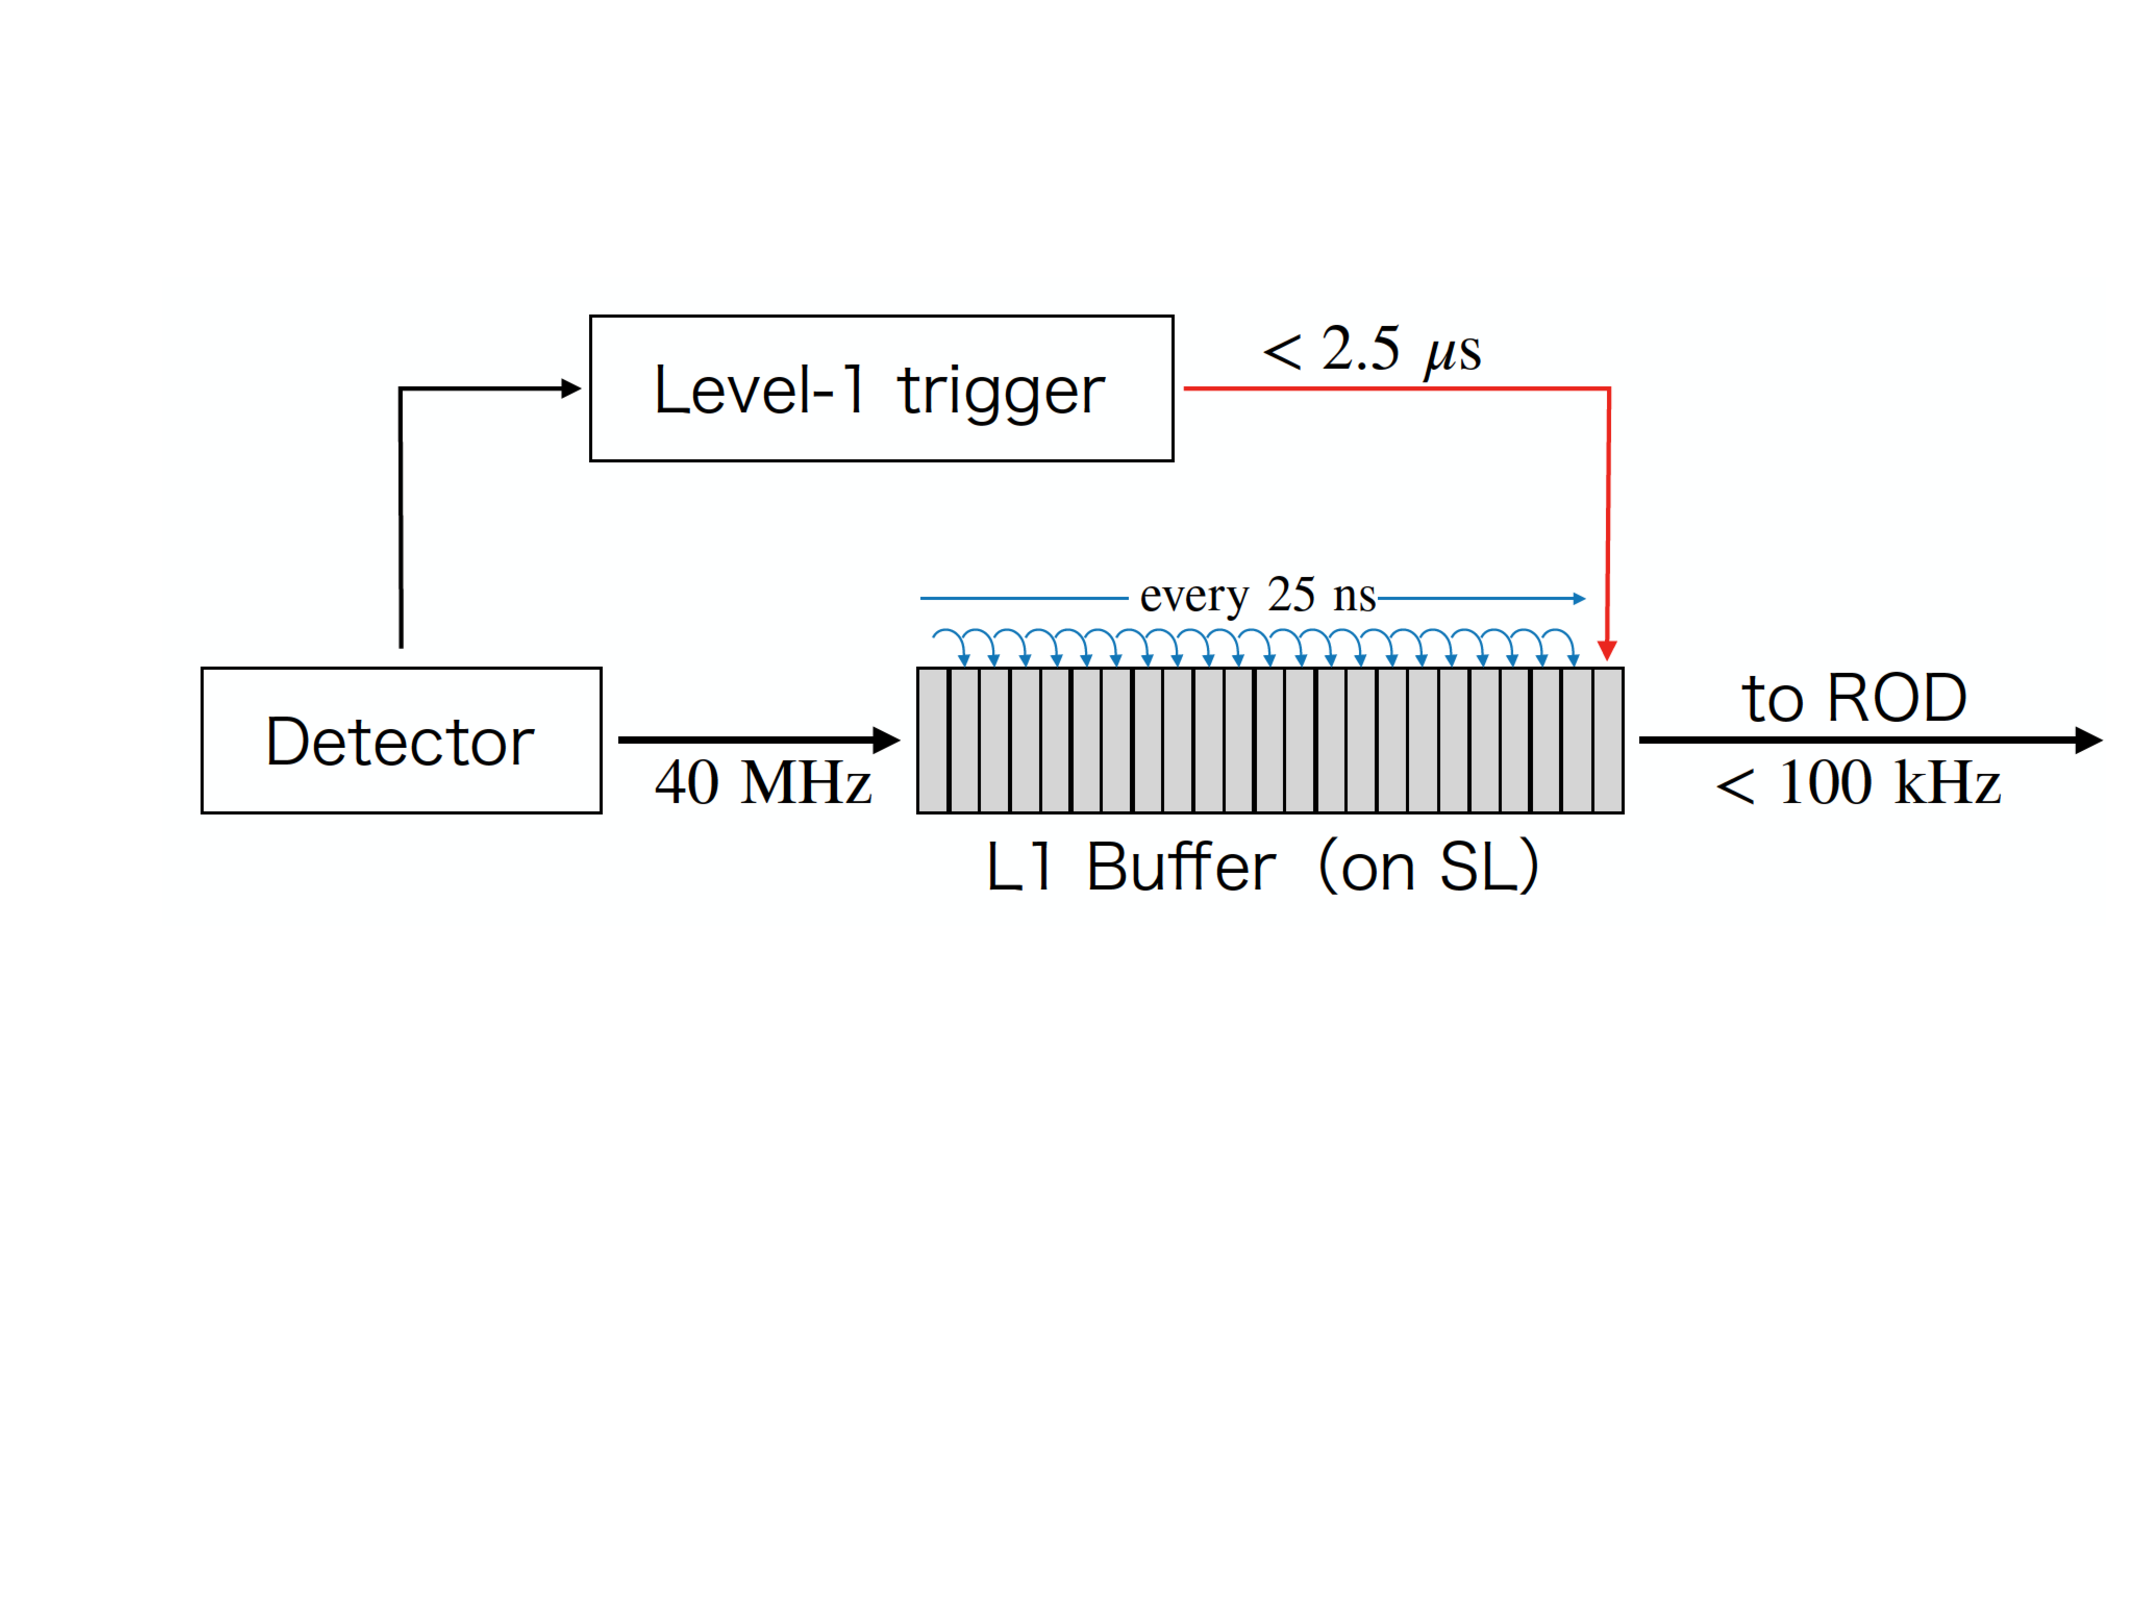
\includegraphics[width=0.95\textwidth,page=1]{img/pdf/pipe.pdf}
        \caption[L1~におけるトリガーシステムの詳細]{L1~におけるトリガーシステムの詳細。40~MHz~での検出器からの情報は~L1~バッファに一時的に保持され、L1~トリガーでの信号の出力を受けたのち、順番に~ROD~へと送信される。}\label{fig:pipe}
\end{figure}
L1~でのトリガー処理はトリガー用ミューオン検出器~(RPC,~TGC)~およびカロリメータによって行われる。それぞれの検出器によって検出された~40~MHz~の頻度で繰り返される陽子バンチ衝突からのヒット信号は、25~ns~おきにL1~バッファに保持され、トリガー処理は情報が保持されている間に行われる。L1~の判定には最大$2.5~\mu\rm{s}$の時間がかかるため、L1~バッファでは最低~100~陽子バンチ分~($25~\rm{ns}\times100=2.5~\mu\rm{s}$)~のデータが保持できるように設定されている。そして決められた遅延時間~(Fixed~Latency)~を経たバンチ衝突のデータに対して、同一のバンチ衝突に対応した~L1~からの信号を受信し、情報の読み出しが行われる。以上のようなトリガー処理システムをパイプライントリガーと呼ぶ。L1~でのイベントの許容レートは~100~kHz~までに設定されており、以上のシステムを通じて~40~MHz~から~100~kHz~以下にまでレートを削減する。

カロリメータおよびミューオン検出器における~L1~の流れについて説明する。カロリメータトリガーでは電子やジェット等の中から高いエネルギーを持つ事象、ミューオントリガーでは高い運動量のミューオンヒットを持つ事象に対してトリガーを行う。L1~は、カロリメータの情報を用いて発行されるトリガー~(L1Calo)、ミューオン検出器の情報を用いて発行されるトリガー~(L1Muon)、それらを組み合わせた複合的なトリガー~(L1Topo)~の~3~種類に分類される。ミューオントリガーではバレル領域とエンドキャップ領域で別々に処理が行われ、L1Muon~の情報は~Muon~to~CTP~Interface~(MUCTPI)~でまとめられる。
そして~L1Calo~と~MUCTPI~でまとめられた~L1Muon~の情報は、Central~Trigger~Processor~(CTP)~へと渡され、それぞれ処理が行われる。

また、L1Calo~と~L1~Muon~の情報は同時に~L1Topo~に送信され、複合的な情報処理が行われる。
L1Topo~においては~L1Calo~と~L1Muon~のトリガーアイテムを組み合わせたトリガーが発行できるだけでなく$\eta$方向、$\phi$方向の位置情報を用いて不変質量を組み、粒子の共鳴に由来することの要求も行うことができる。そして、L1Topo~で処理された情報についても、L1Muon~や~L1Calo~と同様に~CTP~へと送信される。

L1Calo,~L1Muon~および~L1Topo~の情報は、以上の流れから~CTP~に集められ、~512~個の候補選別アルゴリズムを介して事象選別される。CTP~でのトリガー判定によりデータ読み出しが認められた信号に対しては~L1A~(Level-1~Accept)~が発行される。発行された~L1A~は~40~MHz~のクロックとともに~Timing~Trigger~and~Control~(TTC)~システムを経由して各測定器の読み出しシステムに送信される。

L1A~が発行された事象の信号は、情報の読み出しおよび保存を行うために~Read-Out~Driver~(ROD)~に送信される。このときデータは圧縮され、信号情報とともにバンチ交差識別番号~(BCID)~が付与される。BCID~は、LHC~の~25~ns~毎のバンチ衝突に対して、どのバンチに対応しているのかを識別する役割を持つ。ROD~は収集したデータをイベントごとに処理し、BCID~の整合性を確認したのち~Simple~Link~Interface~(S-LINK)~\cite{URL:20}を通して、Read-Out~System~(ROS)~へと情報を送信する。

また、初段トリガーが発行された周辺の位置情報~(Region~of~Interest:~RoI)~は、後段トリガーに渡され事象選別の種として利用される。

\subsubsection{初段トリガーにおけるタイミング合致の重要性}
前節で述べたように~L1~ではパイプライントリガーと呼ばれるシステムを採用している。このトリガーシステムにおいては、異なる検出器ごとの情報を同一のバンチ衝突ごとに対応させ、正しく一致させることが非常に重要となる。検出器は衝突点から最大で約~20~m~の距離に設置されており、ミューオンの検出器到達には最大で約~100~ns~程の時間がかかる。各検出器でのタイミングをそろえるためには詳細な調整が必須である。L1Muon~および~L1Calo~では、各検出器に対し粒子がほぼ光速で到達するということを仮定した上で、基準に定めた陽子バンチ衝突による生成粒子の信号と判断した場合にトリガー判定を行っている。本論文では、トリガー判定を行う上で基準に定められたバンチのことを基準バンチ~(Current~Bunch)~と呼ぶこととする。L1Muon~や~L1Calo~では、基準バンチ由来ではないと考えられるタイミングでの入力情報に対しては、トリガー判定を行うことができない。一方複合的なトリガーである~L1Topo~においては、基準バンチの情報に加えてその次のバンチの情報を組み合わせたトリガー判定を行うことが可能である。本論文では、基準バンチの次の陽子バンチ衝突のことを次バンチ~(Next~Bunch)、また基準バンチの前の陽子バンチ衝突のことを前バンチ~(Previous~Bunch)~と呼ぶ。

以上のように正しくトリガー処理を行うには各検出器において同一バンチの事象を取得することが非常に重要である。

\subsection{後段トリガー}
後段トリガー~(HLT)~では、初段トリガーで出力された~RoI~を種として、ソフトウェアベースのアルゴリズムでオフライン解析に近い粒子の再構成を行う。HLT~では内部飛跡検出器および~MDT~や~CSC~などの精密測定用ミューオン検出器、L1Calo~におけるカロリメータなどの情報を用いて、飛跡再構成および$E_{\rm{T}},~p_{\rm{T}}$の計算をする。L1~で~100~kHz~にまで落とされたイベントレートを~HLT~では数~kHz~にまで削減する。

HLT~は~L1~とは異なり、数~10~ms~から~1~s~程の長い計算時間によってより詳細にトリガー判定を行う。また大量のコンピューティングファーム利用することで精密で膨大な計算を並行して処理することができる。HLT~のアルゴリズムは~Processing~Unit~(PU)~と呼ばれる約~40,000~個のアプリケーションで実行される~\cite{AR:15}。各~PU~は一つの事象を数~100~ms~以内に処理できるように設計されている。PU~の一連の処理においては複数の特徴抽出アルゴリズムが実行される。HLT~において事象がアクセプトされるとオフライン再構成のためにデータを一時ストレージへ送信し、最終的には~CERN~コンピューティングセンターの大規模ストレージシステムに保存する。
